% %                                                                 aa.dem
% % AA vers. 9.1, LaTeX class for Astronomy & Astrophysics
% % demonstration file
%                                                       (c) EDP Sciences
%-----------------------------------------------------------------------
%
% \documentclass[referee]{aa} % for a referee version
%\documentclass[onecolumn]{aa} % for a paper on 1 column  
%\documentclass[longauth]{aa} % for the long lists of affiliations 
%\documentclass[letter]{aa} % for the letters 
%\documentclass[bibyear]{aa} % if the references are not structured 
%                              according to the author-year natbib style

\documentclass[article]{aa}  

%
\usepackage{graphicx}
\usepackage{amsmath,amsfonts,amssymb}
\usepackage{natbib}

%%%%%%%%%%%%%%%%%%%%%%%%%%%%%%%%%%%%%%%%
\usepackage{txfonts}
\usepackage{xcolor}

\usepackage{blindtext}
% \usepackage{siunitx}
% \DeclareSIUnit\arcmin{arcmin}
%%%%%%%%%%%%%%%%%%%%%%%%%%%%%%%%%%%%%%%%
% \usepackage[options]{hyperref}
% To add links in your PDF file, use the package "hyperref"
% with options according to your LaTeX or PDFLaTeX drivers.
\usepackage{float}
%\usepackage{stfloats}
\usepackage{dblfloatfix}
\usepackage{afterpage}
\usepackage{ifthen}
\usepackage[morefloats=12]{morefloats}
\usepackage{threeparttable}

\usepackage{placeins}
\usepackage{multicol}
%\usepackage[breaklinks,colorlinks,citecolor=blue]{hyperref}
% \bibpunct{(}{)}{;}{a}{}{,}
% \usepackage[switch]{lineno}
\definecolor{linkcolor}{rgb}{0.6,0,0}
\definecolor{citecolor}{rgb}{0,0,0.75}
\definecolor{urlcolor}{rgb}{0.12,0.46,0.7}
% \usepackage{hyperref}
\usepackage[breaklinks, colorlinks, urlcolor=urlcolor,
    linkcolor=linkcolor,citecolor=citecolor,pdfencoding=auto]{hyperref}
\hypersetup{linktocpage}
\usepackage{bold-extra}

\usepackage[nameinlink,capitalise]{cleveref}
\Crefname{section}{Sect.}{Sects.}
\Crefname{table}{Table}{Tables}
\Crefname{equation}{Eq.}{Eqs.}
\Crefname{appsec}{appendix}{appendices}

\usepackage{caption}
\usepackage{subcaption}

\DeclareRobustCommand{\ion}[2]{%
\relax\ifmmode
\ifx\testbx\f@series
{\mathbf{#1\,\mathsc{#2}}}\else
{\mathrm{#1\,\mathsc{#2}}}\fi
\else\textup{#1\,{\mdseries\textsc{#2}}}%
\fi}



\def\setsymbol#1#2{\expandafter\def\csname #1\endcsname{#2}}
\def\getsymbol#1{\csname #1\endcsname}

\def\Planck{\textit{Planck}}

\def\HeJT{$^4$He-JT}

\def\allearlypapers{\nocite{planck2011-1.1, planck2011-1.3, planck2011-1.4, planck2011-1.5, planck2011-1.6, planck2011-1.7, planck2011-1.10, planck2011-1.10sup, planck2011-5.1a, planck2011-5.1b, planck2011-5.2a, planck2011-5.2b, planck2011-5.2c, planck2011-6.1, planck2011-6.2, planck2011-6.3a, planck2011-6.4a, planck2011-6.4b, planck2011-6.6, planck2011-7.0, planck2011-7.2, planck2011-7.3, planck2011-7.7a, planck2011-7.7b, planck2011-7.12, planck2011-7.13}}

\def\alltwentythirteenresultspapers{\nocite{planck2013-p01, planck2013-p02, planck2013-p02a, planck2013-p02d, planck2013-p02b, planck2013-p03, planck2013-p03c, planck2013-p03f, planck2013-p03d, planck2013-p03e, planck2013-p01a, planck2013-p06, planck2013-p03a, planck2013-pip88, planck2013-p08, planck2013-p11, planck2013-p12, planck2013-p13, planck2013-p14, planck2013-p15, planck2013-p05b, planck2013-p17, planck2013-p09, planck2013-p09a, planck2013-p20, planck2013-p19, planck2013-pipaberration, planck2013-p05, planck2013-p05a, planck2013-pip56, planck2013-p06b, planck2013-p01a}}

\def\alltwentyfifteenresultspapers{\nocite{planck2014-a01, planck2014-a03, planck2014-a04, planck2014-a05, planck2014-a06, planck2014-a07, planck2014-a08, planck2014-a09, planck2014-a11, planck2014-a12, planck2014-a13, planck2014-a14, planck2014-a15, planck2014-a16, planck2014-a17, planck2014-a18, planck2014-a19, planck2014-a20, planck2014-a22, planck2014-a24, planck2014-a26, planck2014-a28, planck2014-a29, planck2014-a30, planck2014-a31, planck2014-a35, planck2014-a36, planck2014-a37, planck2014-ES}}

\newbox\tablebox    \newdimen\tablewidth
\def\leaderfil{\leaders\hbox to 5pt{\hss.\hss}\hfil}
\def\endPlancktable{\tablewidth=\columnwidth 
    $$\hss\copy\tablebox\hss$$
    \vskip-\lastskip\vskip -2pt}
\def\endPlancktablewide{\tablewidth=\textwidth 
    $$\hss\copy\tablebox\hss$$
    \vskip-\lastskip\vskip -2pt}
\def\tablenote#1 #2\par{\begingroup \parindent=0.8em
    \abovedisplayshortskip=0pt\belowdisplayshortskip=0pt
    \noindent
    $$\hss\vbox{\hsize\tablewidth \hangindent=\parindent \hangafter=1 \noindent
    \hbox to \parindent{$^#1$\hss}\strut#2\strut\par}\hss$$
    \endgroup}
\def\doubleline{\vskip 3pt\hrule \vskip 1.5pt \hrule \vskip 5pt}

\def\L2{\ifmmode L_2\else $L_2$\fi}
\def\dtt{\Delta T/T}
\def\DeltaT{\ifmmode \Delta T\else $\Delta T$\fi}
\def\deltat{\ifmmode \Delta t\else $\Delta t$\fi}
\def\fknee{\ifmmode f_{\rm knee}\else $f_{\rm knee}$\fi}
\def\Fmax{\ifmmode F_{\rm max}\else $F_{\rm max}$\fi}
\def\solar{\ifmmode{\rm M}_{\mathord\odot}\else${\rm M}_{\mathord\odot}$\fi}
\def\Msolar{\ifmmode{\rm M}_{\mathord\odot}\else${\rm M}_{\mathord\odot}$\fi}
\def\Lsolar{\ifmmode{\rm L}_{\mathord\odot}\else${\rm L}_{\mathord\odot}$\fi}
\def\inv{\ifmmode^{-1}\else$^{-1}$\fi}
\def\mo{\ifmmode^{-1}\else$^{-1}$\fi}
\def\sup#1{\ifmmode ^{\rm #1}\else $^{\rm #1}$\fi}
\def\expo#1{\ifmmode \times 10^{#1}\else $\times 10^{#1}$\fi}
\def\,{\thinspace}
\def\lsim{\mathrel{\raise .4ex\hbox{\rlap{$<$}\lower 1.2ex\hbox{$\sim$}}}}
\def\gsim{\mathrel{\raise .4ex\hbox{\rlap{$>$}\lower 1.2ex\hbox{$\sim$}}}}
\let\lea=\lsim
\let\gea=\gsim
\def\simprop{\mathrel{\raise .4ex\hbox{\rlap{$\propto$}\lower 1.2ex\hbox{$\sim$}}}}
\def\deg{\ifmmode^\circ\else$^\circ$\fi}
\def\pdeg{\ifmmode $\setbox0=\hbox{$^{\circ}$}\rlap{\hskip.11\wd0 .}$^{\circ}
          \else \setbox0=\hbox{$^{\circ}$}\rlap{\hskip.11\wd0 .}$^{\circ}$\fi}
\def\arcs{\ifmmode {^{\scriptstyle\prime\prime}}
          \else $^{\scriptstyle\prime\prime}$\fi}
\def\arcm{\ifmmode {^{\scriptstyle\prime}}
          \else $^{\scriptstyle\prime}$\fi}
\newdimen\sa  \newdimen\sb
\def\parcs{\sa=.07em \sb=.03em
     \ifmmode \hbox{\rlap{.}}^{\scriptstyle\prime\kern -\sb\prime}\hbox{\kern -\sa}
     \else \rlap{.}$^{\scriptstyle\prime\kern -\sb\prime}$\kern -\sa\fi}
\def\parcm{\sa=.08em \sb=.03em
     \ifmmode \hbox{\rlap{.}\kern\sa}^{\scriptstyle\prime}\hbox{\kern-\sb}
     \else \rlap{.}\kern\sa$^{\scriptstyle\prime}$\kern-\sb\fi}
\def\ra[#1 #2 #3.#4]{#1\sup{h}#2\sup{m}#3\sup{s}\llap.#4}
\def\dec[#1 #2 #3.#4]{#1\deg#2\arcm#3\arcs\llap.#4}
\def\deco[#1 #2 #3]{#1\deg#2\arcm#3\arcs}
\def\rra[#1 #2]{#1\sup{h}#2\sup{m}}
\def\page{\vfill\eject}
\def\dots{\relax\ifmmode \ldots\else $\ldots$\fi}
\def\WHzsr{\ifmmode $W\,Hz\mo\,sr\mo$\else W\,Hz\mo\,sr\mo\fi}
\def\mHz{\ifmmode $\,mHz$\else \,mHz\fi}
\def\GHz{\ifmmode $\,GHz$\else \,GHz\fi}
\def\mKs{\ifmmode $\,mK\,s$^{1/2}\else \,mK\,s$^{1/2}$\fi}
\def\muKs{\ifmmode \,\mu$K\,s$^{1/2}\else \,$\mu$K\,s$^{1/2}$\fi}
\def\muKRJs{\ifmmode \,\mu$K$_{\rm RJ}$\,s$^{1/2}\else \,$\mu$K$_{\rm RJ}$\,s$^{1/2}$\fi}
\def\muKHz{\ifmmode \,\mu$K\,Hz$^{-1/2}\else \,$\mu$K\,Hz$^{-1/2}$\fi}
\def\MJysr{\ifmmode \,$MJy\,sr\mo$\else \,MJy\,sr\mo\fi}
\def\MJysrmK{\ifmmode \,$MJy\,sr\mo$\,mK$_{\rm CMB}\mo\else \,MJy\,sr\mo\,mK$_{\rm CMB}\mo$\fi}
\def\microns{\ifmmode \,\mu$m$\else \,$\mu$m\fi}
\def\micron{\microns}
\def\muK{\ifmmode \,\mu$K$\else \,$\mu$\hbox{K}\fi}
\def\microK{\ifmmode \,\mu$K$\else \,$\mu$\hbox{K}\fi}
\def\muW{\ifmmode \,\mu$W$\else \,$\mu$\hbox{W}\fi}
\def\kms{\ifmmode $\,km\,s$^{-1}\else \,km\,s$^{-1}$\fi}
\def\kmsMpc{\ifmmode $\,\kms\,Mpc\mo$\else \,\kms\,Mpc\mo\fi}

\providecommand{\sorthelp}[1]{}


% Custom definitions
\newcommand{\mathsc}[1]{{\normalfont\textsc{#1}}}
\newcommand{\dv}[0]{\vec{d}}
\newcommand{\s}[0]{\vec{s}}
\newcommand{\M}[0]{\tens{M}}
\renewcommand{\P}[0]{\tens{P}}
\newcommand{\G}[0]{\tens{G}}
\newcommand{\B}[0]{\tens{B}}
\renewcommand{\a}[0]{\vec{a}}
\newcommand{\n}[0]{\vec{n}}
\renewcommand{\t}[0]{\vec{t}}
\def\Cosmoglobe{\textsc{Cosmoglobe}}
\def\cosmoglobe{\textsc{Cosmoglobe}}
\def\BeyondPlanck{\textsc{BeyondPlanck}}
\def\Planck{\textit{Planck}}
\def\planck{\textit{Planck}}
\def\NPIPE{NPIPE}
\def\npipe{NPIPE}
\def\FIRAS{\textit{FIRAS}}
\def\WMAP{\textit{WMAP}}
\def\COBE{\textit{COBE}}
\def\GAIA{\textit{Gaia}}
\def\gaia{\textit{Gaia}}
\def\Gaia{\textit{Gaia}}
\def\Ha{H$\alpha$}
\def\litebird{\textit{LiteBIRD}}
\def\WISE{WISE}
\def\AKARI{\textit{{AKARI}}}
\def\IRAS{\textit{{IRAS}}}
\def\nside{$N_{\mathrm{side}}$}
\def\wham{\textit{WHAM}}
% \newcommand{\cii}{\ensuremath{\mathsc{C\ ii}}}
\newcommand{\CII}{\ion{C}{ii}}
\newcommand{\cii}{\ion{C}{ii}}
% \newcommand{\CII}{\ensuremath{\mathsc{C\ ii}}}
\def\Commander{\texttt{Commander} }
\def\commanderthree{\texttt{Commander3} }

\def\Tcmb{\ifmmode T_\mathrm{CMB}\else $T_{\mathrm{CMB}}$\fi}
\def\Tcold{\ifmmode T_\mathrm{c}\else $T_{\mathrm{c}}$\fi}
\def\Thot{\ifmmode T_\mathrm{h}\else $T_{\mathrm{h}}$\fi}
\def\Tnear{\ifmmode T_\mathrm{near}\else $T_{\mathrm{near}}$\fi}
\def\scmb{\ifmmode s_\mathrm{CMB}\else $s_{\mathrm{CMB}}$\fi}
\def\squad{\ifmmode s_\mathrm{quad}\else $s_{\mathrm{quad}}$\fi}
\def\ssynch{\ifmmode s_\mathrm{s}\else $s_\mathrm{s}$\fi}
\def\sdust{\ifmmode s_\mathrm{d}\else $s_{\mathrm{d}}$\fi}
\def\ssdust{\ifmmode s_\mathrm{sd}\else $s_{\mathrm{sd}}$\fi}
\def\same{\ifmmode s_\mathrm{AME}\else $s_{\mathrm{AME}}$\fi}
\def\ssrc{\ifmmode s_\mathrm{src}\else $s_{\mathrm{src}}$\fi}
\def\sco{\ifmmode s_\mathrm{CO}\else $s_{\mathrm{CO}}$\fi}
\def\sff{\ifmmode s_\mathrm{ff}\else $s_{\mathrm{ff}}$\fi}
\def\gff{\ifmmode g_\mathrm{ff}\else $g_{\mathrm{ff}}$\fi}
\def\fsynch{\ifmmode f_\mathrm{s}\else $f_{\mathrm{s}}$\fi}
\def\fsd{\ifmmode f_\mathrm{sd}\else $f_{\mathrm{sd}}$\fi}
\def\fame{\ifmmode f_\mathrm{AME}\else $f_{\mathrm{AME}}$\fi}
\def\alphasrc{\ifmmode \alpha_\mathrm{src}\else $\alpha_{\mathrm{src}}$\fi}
\def\bcold{\ifmmode \beta_\mathrm{c}\else $\beta_{\mathrm{c}}$\fi}
\def\bhot{\ifmmode \beta_\mathrm{h}\else $\beta_{\mathrm{h}}$\fi}
\def\bnear{\ifmmode \beta_\mathrm{n}\else $\beta_{\mathrm{n}}$\fi}
\def\bsynch{\ifmmode \beta_\mathrm{s}\else $\beta_{\mathrm{s}}$\fi} 
\def\bsun{\ifmmode \beta_\mathrm{sun}\else $\beta_{\mathrm{sun}}$\fi} 
\def\nuzeros{\ifmmode \nu_{0,\mathrm{s}}\else $\nu_{0,\mathrm{s}}$\fi} 
\def\nuzeroff{\ifmmode \nu_{0,\mathrm{ff}}\else $\nu_{0,\mathrm{ff}}$\fi} 
\def\nuzerocold{\ifmmode \nu_{0,\mathrm{c}}\else $\nu_{0,\mathrm{c}}$\fi}
\def\nuzerohot{\ifmmode \nu_{0,\mathrm{h}}\else $\nu_{0,\mathrm{h}}$\fi}
\def\nuzeronear{\ifmmode \nu_{0,\mathrm{n}}\else $\nu_{0,\mathrm{n}}$\fi} 
\def\nuzeroame{\ifmmode \nu_{0,\mathrm{AME}}\else $\nu_{0,\mathrm{AME}}$\fi} 
\def\nuzerosd{\ifmmode \nu_{0,\mathrm{}}\else $\nu_{0,\mathrm{sd}}$\fi} 
\def\nuzerosrc{\ifmmode \nu_{0,\mathrm{src}}\else $\nu_{0,\mathrm{src}}$\fi} 
\def\nup{\ifmmode \nu_{\mathrm{p}}\else $\nu_{\mathrm{p}}$\fi} 
\def\alphasd{\ifmmode \alpha_{\mathrm{sd}}\else $\alpha_{\mathrm{sd}}$\fi} 
\def\Te{\ifmmode T_{\mathrm{e}}\else $T_{\mathrm{e}}$\fi} 
\def\kB{\ifmmode k_\mathrm{B}\else $k_{\mathrm{B}}$\fi} 

\newcommand{\RS}[1]{\textcolor{red}{RS: #1}}

\definecolor{darkpastelgreen}{rgb}{0.01, 0.75, 0.24}
\usepackage[normalem]{ulem} % enables \sout to strikeout text
\newcommand{\KG}[1]{\textcolor{darkpastelgreen}{(KG: #1)}}

\begin{document} 


%\title{\bfseries{\Cosmoglobe\ DR2. VI. High-resolution templates of hot and cold thermal dust emission derived from Planck HFI}}
\title{\bfseries{\Cosmoglobe\ DR2. VI. Disentangling hot and cold thermal dust emission with Planck HFI}}
%\title{\bfseries{\Cosmoglobe\ DR2. VI. Decomposing thermal dust emission in Planck HFI }}
%\title{\bfseries{\Cosmoglobe\ DR2. VI. High-resolution decomposition of hot and cold thermal dust emission derived from Planck HFI}}


   %This author list corresponds to \title{Author list for L04\_CMB\_Foregrounds\_Extraction}
%Prepared by M. Lopez-Caniego (Marcos.Lopez.Caniego@sciops.esa.int), ESAC/ESA
%This version is from Thu Jul 12 18:11:48 2018 CET
%\subtitle{There are 152 co-authors in this list}
\newcommand{\oslo}[0]{1}
%\newcommand{\MIT}[0]{2}
\newcommand{\milanoA}[0]{2}
\newcommand{\milanoB}[0]{3}
\newcommand{\milanoC}[0]{4}
\newcommand{\triesteB}[0]{5}
\newcommand{\planetek}[0]{6}
\newcommand{\princeton}[0]{7}
\newcommand{\jpl}[0]{8}
\newcommand{\helsinkiA}[0]{9}
\newcommand{\helsinkiB}[0]{10}
\newcommand{\nersc}[0]{11}
\newcommand{\haverford}[0]{12}
\newcommand{\mpa}[0]{13}
\newcommand{\triesteA}[0]{14}
\newcommand{\iia}[0]{2}

\author{\small
J.~R.~Eskilt\inst{\oslo}\thanks{Corresponding author: J.~R.~Eskilt; \url{j.r.eskilt@astro.uio.no}}
\and
K.~Lee\inst{\oslo}
\and
D.~J.~Watts\inst{\oslo}
\and
S.~Nerval\inst{\oslo}
\and
et al.
}
\institute{\small
        Institute of Theoretical Astrophysics, University of Oslo, Blindern, Oslo, Norway \goodbreak
}


   %\institute{Institute of Theoretical Astrophysics, University of Oslo, Blindern, Oslo, Norway}
  
   % Shortened title, author list for top of page 
   \titlerunning{HFI dust templates}
   \authorrunning{.}

   \date{\today} 
   
   \abstract{
	   We present a four-component high-resolution model of thermal dust emission for microwave and infrared frequencies derived from \textit{Planck} HFI, WHAM and \textit{Gaia}. This model is inspired by a joint low-resolution template-based analysis of \textit{Planck} HFI and \textit{COBE}-DIRBE data presented in a companion paper, and the resulting high-resolution model forms the basis for the thermal dust model employed in the \textsc{Cosmoglobe} DR2 reanalysis of \textit{COBE}-DIRBE. The four dust components corresponds to different semi-independent physical effects, referred to as ``cold dust'', ``hot dust'',  ``near dust'', and ``\Ha\ correlated dust''. The \Ha\ dust is a dust extinction component, and has a negative amplitude in the \textit{Planck} HFI bands. The spatial distributions of the near dust and \Ha\ dust components are defined by a \textit{Gaia} 3D extinction model \citep{edenhofer:2024} and the Wisconsin \Ha\ mapper (WHAM; \citealp{wham:2003,2016WHAM}), respectively, while the hot and cold dust components are fit freely pixel-by-pixel to the \textit{Planck} HFI data. 
       %The spectral energy densities (SEDs) of all four components are modelled in terms of modified blackbody (MBB) spectra with a free global temperature, $T$, and spectral index, $\beta$, both of which are fitted globally across the sky. Thus, this dust model has ten global sky parameters (two SED parameters for each dust component plus two global template amplitude parameters) and two amplitudes per pixel, one each for the hot and cold dust; in contrast, previous \textit{Planck} HFI dust models have typically assumed spatially varying MBB temperatures and spectral indices, resulting in three degrees of freedom per pixel. 
       We use a parameter grid search (for global parameters) coupled to a Bayesian Gibbs sampler (for per-pixel parameters) to fit this model to \textit{Planck} HFI data. The best-fit MBB temperature for the hot and cold dust components are $T_{\mathrm{h}} = 30\pm3\,\mathrm{K}$ and $T_{\mathrm{c}} = 11\pm1\,\mathrm{K}$, and the corresponding best-fit spectral indices are $\beta_{\mathrm{h}}\ge1.75$ and $\beta_{\mathrm{c}}=1.85\pm0.10$, respectively. In agreement with the low-resolution template fit analysis of \citet{CG02_05}, we find that the hot dust component is strongly correlated with the FIRAS \ion{C}{ii} map, while the cold dust component is strongly correlated with the HI4PI \ion{H}{i}.
       % and the Dame et al.\ CO $J=1$-0 surveys
 Despite its fewer degrees of freedom per pixel compared to the official \textit{Planck} analysis, we find that this new model performs competitively in terms of overall residuals, capturing between 98.5 and 99.9\,\% of the full-sky dust rms for all channels between 100 and 857\,GHz. When fitting a spatially varying 3-parameter MBB model to the new four-component dust model with isotropic SEDs, we find very similar spatial distributions of $T$ and $\beta$ as in the official \textit{Planck} analysis. We conclude that this new model represents both a statistically more efficient summary of thermal dust in the microwave and far-infrared regimes, as well as a physically more realistic decomposition than the traditional 3-parameter MBB model, due to its strong correlations with well-defined \ion{C}{ii} and \ion{H}{i} line emission tracers. Finally, we expect that the novel templates of hot and cold dust emission presented in this paper may form a key component in future temperature and polarization measurements for projects such as Simons Observatory and \litebird, where high-precision measurements of the dust will be critical for constraining $B$-mode CMB polarization. 
%     and find a strong correlation between the hot dust and singly-ionized-carbon (\ion{C}{II}) emission and the cold dust and the neutral hydrogen emission. It has long been known that the cold dust correlates with the neutral hydrogen emission, however the correlation between hot dust and \ion{C}{II} emission is an exciting development. Since \ion{C}{II} emission is expected in hotter regions of the Milky Way galaxy this is potentially an expected correlation, though historically has been associated only as a gas tracer and remains to be explored further. We find the hot dust to have a MBB temperature of 30~K with $\beta=1.75$, the cold dust temperature of 11.3~K with $\beta=1.75$. The uncertainty in the gain for the \planck\ HFI 545 and 857 GHz bands contribute heavily to the uncertainty in these parameters, motivating a future \planck\ HFI end-to-end reanalysis. 
   % Using the final \Planck\ data release, PR4, we generate updated dust template models following a new four component model with nearby dust, dust extinction, cold dust and hot dust. The hot and cold dust have free amplitudes per pixel but fixed global temperature and spectral index $\beta$. The nearby dust is initialized with a template of dust absorption from the GAIA star catalogue, produced by \cite{edenhofer:2024}. Finally, the dust extinction is initialized with a template from the \wham\ survey. These are further constrained using the Commander Gibbs sampling framework to constrain the dust models spectral energy distributions (SEDs). For this analysis we use the \Planck\ HFI single horn channels, namely 100~GHz, 143~GHz, 217~GHz, 353~GHz, 545~GHz, and 857~GHz, as well as \FIRAS\ bands 857, 1251, 1809, 2081, 2135 and 2802 GHz. The SEDs are modelled with a spatially constant standard modified blackbody (MBB) distribution (i.e. a globally constant temperature and $\beta$ for each dust component), but with a spatially varying amplitude in the case of the cold and hot dust, and a spatially constant (fit to a template) amplitude in the case of the nearby dust and dust extinction. We find that the hot dust correlates strongly with \ion{C}{ii} emission and is found to have . The dust extinction template is the \ion{H}{$\alpha$} emission and is found to have . The cold dust finally is found to have,  and also correlates strongly with the neutral hydrogen mapped with HI4PI.
   }
   \keywords{ISM: general - Cosmology: observations, diffuse radiation - Galaxy: general}

   \maketitle
\setcounter{tocdepth}{2}

\tableofcontents
   
% INTRODUCTION
%-------------------------------------------------------------------
\section{Introduction}

% \begin{itemize}
%     \item DIRBE DR2 analysis goals
%     \item Big picture
%     \item Why are we doing this (issues with Planck dust model, results from Eirik)
% \end{itemize}

%overview, a bit why we do what we do?
Observing the Universe through a screen of foregrounds offers opportunities for both discovery and frustration. The foregrounds ultimately complicate our understanding of the backgrounds, and when poorly understood, lead to misinterpretations or increased noise on signals from those backgrounds in turn. However, a better understanding of the foregrounds allows us to uncover the physics permeating matter on all scales, from within our solar system, to the Milky Way, to distant galaxies, while simultaneously allowing us to better observe the far away signals of, for example, the cosmic microwave background (CMB) and the cosmic infrared background (CIB), among others. Of particular interest to this paper and the cosmology community at large is the composition of thermal dust. Thermal dust represents a significant noise contribution to future measurements of primordial polarization $B$-modes, predicted to have been produced by gravitational waves during inflation and is the goal measurement for several ongoing or upcoming CMB experiments \citep{litebird2022,SO2019}. 

There are several types of matter within the Milky Way galaxy. Aside from the aforementioned dust there is additionally gas (generating emission lines such as singly ionized carbon (\ion{C}{ii}), hydrogen emission lines such as \Ha, neutral hydrogen (\ion{H}{i}), carbon monoxide (CO) and many more), stars, spinning dust, ions and electrons (interacting with magnetic fields to produce synchrotron and free-free radiation) and dark matter (only thus far interacting gravitationally). Each of these foregrounds map out relevant regions of the Milky Way and the interstellar medium (ISM). Since dust and gas live side-by-side, it is natural that one may trace the other, and indeed it is known that the neutral hydrogen signature (as observed by e.g. HI4PI, \citealt{HI4PI2016}) and CO \citep{dame2001} trace cold dust. Another observable we can use is the reddening or extinction measurements of starlight, which occur when their light passes through dust regions \citep{lenz:2017,edenhofer:2024}. Finally, as recently shown by \cite{CG02_05}, the \ion{C}{ii} emission lines, as measured by FIRAS, trace hot dust regions. Before \cite{CG02_05} it was not known to us that \ion{C}{ii} could be used as a dust tracer, however, as it is expected to be present in hot regions of the Milky Way galaxy, it is not unexpected that this acts as a tracer for the hot dust.\footnote{It has also been hypothesized that dust may be responsible for the \ion{C}{ii} deficit in luminous-FIR galaxies \citep{2020CII,2017Herschel_FIR_CII}.} 

The dust in the Milky Way will act to absorb radiation at frequencies close to its particle size and re-emit as an imperfect blackbody. Historically, this has been modeled with a modified blackbody spectrum (MBB) characterized by a temperature, $T$, and a `tilt' to the spectrum, called the spectral index and denoted by $\beta$. These, with an amplitude ($a$), define how much radiation at a particular frequency, $\nu$, is produced (see \cite{Hensley2023} for a recent review of dust and the interstellar medium). During the \planck\ analysis the dust in the Milky Way was modelled with a single modified blackbody fit for each pixel, or direction, in the sky. However, it is known that there are different dust populations \cite{finkbeiner1999}, and with enough data it should be possible to make distinct templates modelling each independently. The challenge \planck\ faced with their analysis, of course, was that there was insufficient data to distinguish these populations; there is a clear degeneracy between the dust temperature and the dust spectral index maps \citep{planck2014-a12}.

Thus, we employ maps produced by \cite{edenhofer:2024} of the nearby dust in the Milky Way,  and the \Ha\ maps produced by the Wisconsin H-$\alpha$ mapper (WHAM) \citep{wham:2003,2016WHAM}, which was shown in \cite{CG02_05} to map out a dust extinction component in the \planck\ HFI and DIRBE bands. We use these two data sets as templates, fixing the relative amplitudes between pixels, but allowing the overall amplitudes of the maps, as well as the temperature and spectral indices, to vary globally (changing the relative amplitudes between the frequencies). We also have two additional dust components, here called the hot and the cold dust, which have freely varying amplitudes per pixel, but a global temperature and spectral index. Compared to the previous \planck\ analysis, which had three free parameters per pixel, we instead have ten global parameters, with only two free parameters per pixel, i.e. for the hot and cold amplitudes. At high resolutions this represents a significant reduction in the number of parameters to fit, and has the additional benefit that we see clear correlations between the cold dust and the HI4PI maps (a known cold dust tracer), and the hot dust and \ion{C}{ii}. 

This paper is one of seven companion papers from the \cosmoglobe\ data release 2 \citep[DR2;][]{CG02_01} reanalyzing the \COBE-DIRBE data \citep{hauser1998}. Of particular interest for this release is new constraints on the spectrum of the CIB \citep{CG02_03}, and better constraints on all foregrounds ranging from the microwave to the infrared, including zodiacal light \citep{CG02_02} and stars \citep{CG02_04}. 
%paragraph mimicking the Dust05 
In a companion dust paper, by \cite{CG02_05}, we perform a linear regression analysis of \planck\ HFI 353-857~GHz and DIRBE 3.5-100~$\mu$m data to a five template dust model with minimal assumptions. This further demonstrates that there are distinct dust populations that can be modelled independently with sufficient data sets at a wide range of frequencies, and revealed the new dust tracer, the \ion{C}{ii} line emission, tracing hot dust. 
 Building off of that work, in the current paper we perform a Bayesian analysis of the \planck\ HFI data, deriving high-resolution templates of \ion{H}{i} and \ion{C}{ii} correlated dust components, as well as the \Ha\ and nearby dust template fits. Finally, in \cite{CG02_07} this new dust model is applied to the \COBE-DIRBE data. 

%what is gonna happen in this paper
The rest of the paper is organized as follows. In \cref{sec:data} we discuss the data sets we use for this analysis, including HFI, FIRAS and ancillary data sets. We next discuss the sky and data model in \cref{sec:skymodel}. In \cref{sec:method} we discuss our methodology, primarily the Gibbs sampling and grid search tests, along with the optimization strategy used for the grid search. In \cref{sec:results} we present the best fit results for our new thermal dust model. In \cref{sec:gof} we discuss the goodness of fit of the model, and in \cref{sec:correlations} the correlations with external line emission maps. In \cref{sec:mbb} we compare to the previous \planck\ results and show the MBB fit to the multi-component dust model. Finally, in \cref{sec:conc} we will present our conclusions. In \cref{app:residuals}, \cref{app:GridSearchTests} and \cref{app:dustCharacterization} we include supplementary details regarding the residuals, the grid search and the dust characterization for clarity.

\begin{figure}
	\centering
	\includegraphics[width=0.9\linewidth]{figures/all_masks_descriptive.pdf}
	\caption{All masks used for different stages of the analysis. \emph{Gains:} Mask used during the gain calculations for the 857~GHz maps. \emph{FIRAS:} Mask used during the FIRAS Gibbs sampling routine for the monopoles, dipoles and $\chi^2$ evaluation. \emph{Gibbs sampl:} Mask used during the HFI Gibbs sampling routine for the monopoles, dipoles and $\chi^2$ evaluation. {Grid search:} Mask used to compare the $\chi^2$ in the grid search.}
	\label{fig:all_masks}
\end{figure}


\section{Data}
\label{sec:data}
In \cite{CG02_05} we compute a linear fit to the DIRBE data, finding a good fit to a five template fit dust model.
To build on this work we will use the \planck\ PR4 data, several FIRAS maps, and additional ancillary data to best break degeneracies and constrain the new high resolution four component dust model. We discuss some of the masks used in \cref{sec:masks}. 
\subsection{\Planck\ HFI}
\label{sec:planckhfi}
The \planck\ PR4 (also known as \npipe) maps are the final \planck\ data release, improving on previous data releases by jointly analyzing the low-frequency instrument (LFI) and the  high-frequency instrument (HFI) data in a single pipeline, in addition to several other improvements (for details see \cite{planck2020-LVII}). 
For this analysis we use the single-bolometer HFI maps; HFI because of its strong constraining power on the dust and single-bolometer to better control the gain fluctuations and model components such as the CO-emission.\footnote{The 100~GHz and 143~GHz maps are at an \nside\ of 2048, the other frequencies are at an \nside\ of 4096.} 
In a pre-processing step we correct all maps for the zodiacal light emission, using the \Planck\ PR2 zodiacal light model \citep{planck2014-a09, planck2013-pip88, maris2006c}, and apply a correction for the CIB to the 857, 545 and 353 GHz maps from the GNILC CIB results \cite{planck2016-XLVIII}.
We apply a scaling correction to the root-mean squared (RMS) maps, such that the tail of the spectra matches the white-noise level from the RMS maps.\footnote{The published individual bolometer frequency RMS maps have known residual offsets from the analysis pipeline, evident when comparing the map and RMS power-spectra.} 
%Finally, the gain for 545 GHz is set to a static shift of 0.99145 for 545-1, 1.00487 for 545-2, and 1.00830 for 545-4 (see \cref{tab:gains}) and we sample the 857~GHz gains.\footnote{The uncertainty on the 545~GHz gain is 2\% from the \NPIPE\ analysis.} All other gains and bandpass' are fixed to the \NPIPE\ values. 

\subsection{FIRAS}
\label{sec:firas}
FIRAS was an early cosmology telescope with the goal of measuring the blackbody spectrum of the CMB to unprecedented precision \citep{fixsen1997}. As such the FIRAS maps have very low calibration uncertainties, and so we use them to help calibrate the map amplitudes. The FIRAS 857, 1251, 1809, 2081, 2135 and 2802 GHz maps are used for this analysis in conjunction with the HFI maps. 

\subsection{Ancillary data}
\label{sec:otherdata}
The nearby dust relative amplitudes are fixed to the \GAIA-based dust extinction template by \citet{edenhofer:2024}, which covers distances up to 1.25 kpc. This primarily uses \GAIA\ distances and extinction estimates to build a 3D map of the nearby dust from \citet{2023Zhang}, which also leverages the two micron all sky survey (2MASS), the wide-field infrared survey explorer (WISE and unWISE), the large sky area multi-object fibre spectroscopic telescope (LAMOST). We use the total integrated dust map for our model in this analysis. 
Additionally, we use the Wisconsin H-$\alpha$ mapper data as a template for the \Ha\ correlated dust, and the results from \citep{CG02_05} as the fiducial values for the \Ha\ MBB, since we find that it is poorly constrained by the \planck\ bands (see \cref{sec:results}). As with DIRBE, the \Ha\ dust is a small extinction component in the \Planck\ bands.  
When considering our summary statistics in \cref{sec:correlations} we compare the new dust templates with the 157.7$\mu$m \ion{C}{ii} line emission as measured by the FIRAS \ion{C}{ii} map, available on the LAMBDA\footnote{\url{lambda.gsfc.nasa.gov}} website, and to the HI4PI data \citep{HI4PI2016}. 

\subsection{Masks}
\label{sec:masks}
When computing the $\chi^2$ for the grid search (see \cref{sec:statistics}) we apply a mask to remove the extreme outliers in the $\chi^2$ map, as can be seen in yellow in \cref{fig:all_masks}, this has an $f_\mathrm{sky}$ of 99\% (masking only 1\% of the sky).
During the Gibbs sampling (see \cref{sec:sampling}), we apply a 30 degree galactic plane mask to the FIRAS maps when computing monopole and dipole estimates (representing an $f_\mathrm{sky}$ of 50\%), and a large galactic cut (of areas with the largest foregrounds) to the HFI maps with an $f_\mathrm{sky}$ of 48\%, as can be seen in dark and light purple in \cref{fig:all_masks}. When estimating the gain for the 857~GHz maps we employ a small mask of $f_\mathrm{sky}$ of 95\%, as seen in orange in \cref{fig:all_masks}. The component estimation (as discussed in \cref{sec:skymodel}) were all done using the full sky.

% \begin{figure}
% 	\centering
% 	\includegraphics[width=0.9\linewidth]{figures/all_masks_descriptive.pdf}
% 	\caption{All masks used for different stages of the analysis. \emph{Gains:} Mask used during the gain calculations for the 857~GHz maps. \emph{FIRAS:} Mask used during the FIRAS Gibbs sampling routine for the monopoles, dipoles and $\chi^2$ evaluation. \emph{Gibbs sampl:} Mask used during the HFI Gibbs sampling routine for the monopoles, dipoles and $\chi^2$ evaluation. {Grid search:} Mask used to compare the $\chi^2$ in the grid search.}
% 	\label{fig:all_masks}
% \end{figure}

% To constrain the four-component dust model we employ several techniques. 
% - Gibbs sampling, 
% - grid search




% \RS{fis this}
 
% We build off the work in \cite{CG02_05}, by using several data sets, discussed in \cref{sec:data}, and using two techniques, Gibbs sampling, discussed in \cref{sec:sampling}, and a parameter grid search, discussed in \cref{sec:statistics}. 
% Additionally, we will discuss the sky model and the data model used for this analysis in \cref{sec:skymodel}.

\section{Data model and posterior distribution}
\label{sec:skymodel}

The data model for this analysis can be written as
\begin{align}
    \vec{d}=&\mathsf{G}\left[\mathsf{B}\sum_s \mathsf{M}_{s}\vec{a}_{s}\right]+\vec{n}\nonumber\\
    \equiv & \vec{s}+ \vec{n}
\label{equ:dataModel}
\end{align}
where $\mathsf{G}$ is the instrumental gain matrix for each detector, $\mathsf{B}$ the instrumental beam convolution, $\mathsf{M}_{s}a_{s}$ is the foregrounds mixing matrix which extrapolates the sky component $s$ to the given frequency (including bandpass and the spectral shape of the particular component) and amplitudes $\vec{a}_{s}$ per pixel for the various sky components ($s$), and $\vec{n}$ is the noise. 

The \planck\ HFI bands contain several relevant foregrounds in addition to dust, such as free-free, CO, and the CMB. 
 As such, the temperature model used for this analysis may be written as a vector per pixel
\begin{align}
    \vec{s}_\nu=&u_\nu 
    \left[\vphantom{\left(\frac{\nu}{\nu_\mathrm{d}}\right)^{\beta_\mathrm{d}+1}}\vec{a} _\mathrm{cmb}\gamma(\nu) \right. &\mathrm{(CMB)} \nonumber \\
    &+\left(\frac{\nu_{0,\mathrm{ff}}}{\nu}\right)^2\frac{g_\mathrm{ff}(\nu;T_\mathrm{e})}{g_\mathrm{ff}(\nu_{0,\mathrm{ff}};T_\mathrm{e})}\vec{t}_\mathrm{ff} & \textrm{(Free-free)}\nonumber \\
    &+\vec{a}_\mathrm{c}\left(\frac{\nu}{\nu_\mathrm{c}}\right)^{\beta_\mathrm{c}+1}\left(\frac{e^{h\nu_\mathrm{c}/k_\mathrm{B}T_\mathrm{c}}-1}{e^{h\nu/k_\mathrm{B}T_\mathrm{c}}-1}\right) &\textrm{(Cold\ dust)}\nonumber \\
    &+\vec{a}_\mathrm{h}\left(\frac{\nu}{\nu_\mathrm{h}}\right)^{\beta_\mathrm{h}+1}\left(\frac{e^{h\nu_\mathrm{h}/k_\mathrm{B}T_\mathrm{h}}-1}{e^{h\nu/k_\mathrm{B}T_\mathrm{h}}-1}\right) &\textrm{(Hot\ dust)}\nonumber \\
    &+a_\mathrm{near}\vec{t}_\mathrm{near}\left(\frac{\nu}{\nu_\mathrm{near}}\right)^{\beta_\mathrm{near}+1}\left(\frac{e^{h\nu_\mathrm{near}/k_\mathrm{B}T_\mathrm{near}}-1}{e^{h\nu/k_\mathrm{B}T_\mathrm{near}}-1}\right)&\textrm{(Near\ dust)}\nonumber \\
    &+a_\mathrm{H\alpha}\vec{t}_\mathrm{H\alpha}\left(\frac{\nu}{\nu_\mathrm{H\alpha}}\right)^{\beta_\mathrm{H\alpha}+1}\left(\frac{e^{h\nu_\mathrm{H\alpha}/k_\mathrm{B}T_\mathrm{H\alpha}}-1}{e^{h\nu/k_\mathrm{B}T_\mathrm{H\alpha}}-1}\right) &\textrm{(H$\alpha$\ dust)}\nonumber \\
&+\vec{a}^{100}_\mathrm{co}h_\nu^{100}+\vec{a}^{217}_\mathrm{co}h_\nu^{217} +\vec{a}^{353}_\mathrm{co}h_\nu^{353}\left. \vphantom{\left(\frac{\nu}{\nu_\mathrm{d}}\right)^{\beta_\mathrm{d}+1}}\right] & \textrm{(CO)}\nonumber\\
    &+m_\nu &\textrm{(Monopole)}
\label{equ:model}
\end{align}
where $u_\nu$ is a unit scaling conversion factor to go from brightness temperature to thermodynamic temperature, $\gamma(\nu)$ represents the CMB fluctuation spectrum in brightness temperature (including the CMB dipole and associated effects),
$\vec{a}_{s}$ for $s\in (\mathrm{c,h,co})$ are the amplitudes sampled per-pixel for the CMB ($\mathrm{cmb}$), cold dust ($\vec{a}_\mathrm{c}$), hot dust ($\vec{a}_\mathrm{h}$), and the CO lines (($\vec{a}^{\{100,217,353\}}_\mathrm{co}$)). We keep the CO line-ratios ($h_\nu^{\{100,217,353\}}$) constant for this analysis from the \planck\ results \cite{planck2020-LVI}. We also keep the free-free  fixed due to the low constraining power of the HFI bands on the free-free component. The template we use has electron temperature ($T_e$) of 7000 K and amplitudes ($\vec{t}_\mathrm{ff}$) and Gaunt factor ($g_\mathrm{ff}$) from the Beyond Planck analysis \cite{bp01}. $a_\mathrm{near}$ and $a_\mathrm{H\alpha}$ are amplitude scale value applied to templates ($\vec{t}_\mathrm{near}$ based on \cite{edenhofer:2024} and $\vec{t}_\mathrm{H\alpha}$ based on \cite{wham:2003,2016WHAM}) for the nearby dust ($\mathrm{near}$) and \Ha\ correlated (\Ha) dust respectively.   
Finally, the monopoles ($m_\nu$) are sampled for each frequency band. As mentioned in \cref{sec:planckhfi} we have corrected the maps for the CIB and zodiacal light, so these are not included here, as well as synchrotron and anomalous microwave emission (AME) which are subdominant in the HFI frequency range. 
Note that while in \cite{CG02_05} we fit a five-component dust model, of which one is the carbon monoxide correlated dust, in this case the true CO emission is highly correlated with the CO dust component and since we don't include the DIRBE sensitive CO channels it is effectively merged with the cold dust component. 

\begin{figure}[tbp]
    \centering
    \includegraphics[width=0.85\linewidth]{figures/cmb_map.pdf}
    \includegraphics[width=0.85\linewidth]{figures/ff_map.pdf}
    \includegraphics[width=0.85\linewidth]{figures/co100_map_nc.pdf}
    \includegraphics[width=0.85\linewidth]{figures/co217_map_nc.pdf}
    \includegraphics[width=0.85\linewidth]{figures/co353_map.pdf}
    \caption{Sky model amplitude maps corresponding to the baseline thermal dust model. From top to bottom, the panels show CMB, free-free, CO $J=$1-0, CO $J=$2-1, and CO $J=3-2$. All maps are smoothed to a common resolution of  80$^\prime$ FWHM. }
    \label{fig:SkyModel}
\end{figure}

% \subsection{FIRAS}
% \label{sec:firas}
% FIRAS was an early cosmology telescope with the goal of measuring the blackbody spectrum of the CMB to unprecedented precision \citep{fixsen1997}. As such the FIRAS maps have very low calibration uncertainties, and so we use them to help calibrate the map amplitudes. The FIRAS 857, 1251, 1809, 2081, 2135 and 2802 GHz maps are used for this analysis in conjunction with the HFI maps. 

% \begin{figure*}[htbp]
%     \centering
%     \includegraphics[width=\linewidth]{figures/SEDGrid_withOneColourbar.pdf}
%     \caption{Contour plot of relevant statistical tests and $\chi^2$ for each dust model SED. Maps of a subset of the grid points can be found in \cref{app:GridSearchTests}. }
%     \label{fig:SEDGridContours}
% \end{figure*}

% \begin{figure}[htbp]
%     \centering
%     \includegraphics[width=\linewidth]{figures/Amp_chisq_near.pdf}\\
%     \includegraphics[width=\linewidth]{figures/Amp_chisq_Ha.pdf}
%     \caption{$\chi^2$ as a function of near (\emph{top}) and \Ha\ correlated (\emph{bottom}) dust amplitude scale. Note that the range of the scale of the $\chi^2$ axes are very small. }
%     \label{fig:SEDGridAmplitude}
% \end{figure}


% \subsection{Ancillary data}
% \label{sec:otherdata}
% The nearby dust relative amplitudes are fixed to the \GAIA-based dust extinction template by \citet{edenhofer:2024}, which covers distances up to 1.25 kpc. This primarily uses \GAIA\ distances and extinction estimates to build a 3D map of the nearby dust from \citet{2023Zhang}, which also leverages the two micron all sky survey (2MASS), the wide-field infrared survey explorer (WISE and unWISE), the large sky area multi-object fibre spectroscopic telescope (LAMOST). We use the total integrated dust map for our model in this analysis. 
% Additionally, we use the Wisconsin H-$\alpha$ mapper data as a template for the \Ha\ correlated dust, and the results from \citep{CG02_05} as the fiducial values for the \Ha\ MBB, since we find it is poorly constrained by the \planck\ bands (see \cref{sec:results}). As with DIRBE, the \Ha\ dust is a small extinction component in the \Planck\ bands.  
% When considering our summary statistics in \cref{sec:correlations} we compare the new dust templates with the 157.7$\mu$m \ion{C}{ii} line emission as measured by the FIRAS \ion{C}{ii} map, available on the LAMBDA website.\footnote{\url{lambda.gsfc.nasa.gov}}, and to the HI4PI data \citep{HI4PI2016}. 

% \subsection{Masks}
% \label{sec:masks}
% When computing the $\chi^2$ for the grid search (see \cref{sec:statistics}) we apply a mask to remove the extreme outliers in the $\chi^2$ map, as can be seen in yellow in \cref{fig:all_masks}, this has an $f_\mathrm{sky}$ of 99\% (masking only 1\% of the sky).
% During the Gibbs sampling (see \cref{sec:sampling}), we apply a 30 degree galactic plane mask to the FIRAS maps when computing monopole and dipole estimates (representing an $f_\mathrm{sky}$ of 50\%), and a large galactic cut (of areas with the largest foregrounds) to the HFI maps with an $f_\mathrm{sky}$ of 48\%, as can be seen in dark and light purple in \cref{fig:all_masks}. When estimating the gain for the 857~GHz maps we employ a small mask of $f_\mathrm{sky}$ of 95\%, as seen in orange in \cref{fig:all_masks}. The component estimation (as discussed in \cref{sec:skymodel}) were all done using the full sky.


% To constrain the four-component dust model we employ several techniques. 
% - Gibbs sampling, 
% - grid search




% \RS{fis this}
 
% We build off the work in \cite{CG02_05}, by using several data sets, discussed in \cref{sec:data}, and using two techniques, Gibbs sampling, discussed in \cref{sec:sampling}, and a parameter grid search, discussed in \cref{sec:statistics}. 
% Additionally, we will discuss the sky model and the data model used for this analysis in \cref{sec:skymodel}.

\begin{table}[tbp!]
\begingroup
\newdimen\tblskip \tblskip=5pt
\nointerlineskip
\vskip -3mm
\footnotesize
\setbox\tablebox=\vbox{
\halign{\tabskip 0pt \hbox to 0.6333\linewidth{#\leaderfil}\tabskip 0pt&\hbox to 0.3167\linewidth{\hfil#}\tabskip 0pt\cr
\noalign{\doubleline\vskip 1pt}
\omit\hbox to 1in{Band\hfil}& Gain scale\cr
\noalign{\vskip 4pt\hrule\vskip 6pt}
\noalign{\vskip 3pt}
545-1& $ 0.99145 $\cr
\noalign{\vskip 3pt}
545-2& $ 1.00487 $\cr
\noalign{\vskip 3pt}
545-4& $ 1.00830 $\cr
\noalign{\vskip 3pt}
857-1& $ 0.99362 $\cr
\noalign{\vskip 3pt}
857-2& $ 1.10242 $\cr
\noalign{\vskip 3pt}
857-3& $ 1.02393 $\cr
\noalign{\vskip 3pt}
857-4& $ 1.13470 $\cr
\noalign{\vskip 3pt}
\noalign{\vskip 3pt\hrule\vskip 4pt}}}
\endPlancktable
\endgroup
\caption{Gain values for 545 and 857~GHz bands. The gains for 857 GHz were sampled during the Gibbs loop, the 545 gains were set during initial testing.}
\label{tab:gains}
\end{table}



\begin{table}[tbp!]
\begingroup
\newdimen\tblskip \tblskip=5pt
\nointerlineskip
\vskip -3mm
\footnotesize
\setbox\tablebox=\vbox{
     \newdimen\digitwidth
 \setbox0=\hbox{\rm 0}
 \digitwidth=\wd0
 \catcode`*=\active
 \def*{\kern\digitwidth}
%
  \newdimen\dpwidth
  \setbox0=\hbox{.}
  \dpwidth=\wd0
  \catcode`!=\active
  \def!{\kern\dpwidth}

\halign{\tabskip 0pt \hbox to 0.4750\linewidth{#\leaderfil}\tabskip 0pt&\hbox to 0.175\linewidth{\hfil#\hfil}\tabskip 0pt&\hbox to 
0.175\linewidth{\hfil#\hfil}\tabskip 0pt&\hbox to 0.175\linewidth{\hfil#}\tabskip 0pt\cr
\noalign{\doubleline\vskip 1pt}
\omit\hbox to 1in{Component\hfil}& $T$ (K) & $\beta$ &$a$ scale\cr
\noalign{\vskip 4pt\hrule\vskip 6pt}
\noalign{\vskip 3pt}
Cold dust& $ 11\pm1 $ & $ 1.85 \pm 0.1$ & -\cr
\noalign{\vskip 3pt}
Hot dust& $ 30 \pm 3$ & $ \ge 1.75 $ & -\cr
\noalign{\vskip 3pt}
\Ha\ dust& $ 17.8^\mathrm{a} $ & $ 2.62^\mathrm{a} $ & $1^\mathrm{a}$\cr
\noalign{\vskip 3pt}
Nearby dust& $ 18 \pm 2$ & $ 1.7 \pm 0.1 $& $\le 1^\mathrm{b}$\cr
\noalign{\vskip 3pt}
\noalign{\vskip 3pt\hrule\vskip 4pt}}}
\endPlancktable
\endgroup
\caption{Parameters fit in the grid search. See 
\cref{fig:dustSED} the spectral energy distribution of the dust components and \cref{fig:SEDGridContours} and \cref{fig:SEDGridAmplitude} for the grid search contours. }
\tablewidth=\columnwidth
\tablenote {{\rm a}} {\it \footnotesize{\Ha\ dust is poorly constrained by the HFI data and so are set to the DIRBE fits \citep{CG02_05}.}}\par
\tablenote {{\rm b}} {\it \footnotesize{The amplitude scale for the fiducial value is scaled to 1 and samples in \cref{fig:SEDGridAmplitude} are sampled around this scale.}}\par
\label{tab:SEDs}
\end{table}


\begin{figure}[htbp]
    \centering
    \includegraphics[width=0.9\linewidth]{figures/SED_rmsAmp_logyx.pdf}
    \caption{Spectral energy distribution for the four dust components across the HFI bands. Note that the \Ha\ dust is a negative amplitude since it is an extinction component, but the absolute value is plotted for clarity. Lower bound is set by a 70\% $f_\mathrm{sky}$ and upper bound by a 94\% $f_\mathrm{sky}$. }
    \label{fig:dustSED}
\end{figure}


\begin{figure*}[t]
    \centering
\includegraphics[width=0.8\linewidth]{figures/dustComp_coldDust.pdf}
\includegraphics[width=0.8\linewidth]{figures/dustComp_hotDust.pdf}
\includegraphics[width=0.4\linewidth]{figures/dustComp_Himap.pdf}
\includegraphics[width=0.4\linewidth]{figures/dustComp_firasCII.pdf}
    \caption{DR2 Cold and hot dust components (top panels) as compared with relevant tracers \ion{H}{i} and \ion{C}{ii} (bottom panels).}
    \label{fig:dust_figures}
\end{figure*}

\begin{figure*}[t]
    \centering
    \includegraphics[width=0.85\linewidth]{figures/AvgDust_Grid_plotres.pdf}
    \caption{Left most column shows the sum of the dust maps averaged for each band (plus the residuals), and the middle column the corresponding residuals (with the same color bar range). The final column shows the residuals with the color bar scaled down by a factor of 100 to more easily see the structure in the residuals. The structure in the residuals indicates there may be still some zodiacal light, and that the CO lines, particularly in the 100~GHz bands could be improved. Additionally, it appears that the 545~GHz gain may also be able to be improved upon in future analysis. All the maps have been smoothed by 2 degrees for clarity.}
    \label{fig:MapsVsResiduals}
\end{figure*}


\begin{figure}[t]
    \centering
    \includegraphics[width=\linewidth]{figures/efficiency_avg.pdf}
    \caption{Efficiency of the dust model representing the data. Taking the input map minus the non-dust components (e.g. CMB, free-free, CO) squared minus the residuals squared, divided by the residuals squared and summed across the map we can measure how much of the signal is represented by the model and find that it is greater than 99\% across all HFI bands. This can also be seen clearly in \cref{fig:MapsVsResiduals} where it is clear that the residuals are around 100 times smaller than the dust signal at each band.
	% \\
	%\textbf{Duncan question: how much does the efficiency depend on the pivot / signal-to-noisse?}
	}
    \label{fig:efficiency}
\end{figure}


% \section{Data model and posterior distribution}
% \label{sec:skymodel}

% The data model for this analysis can be written as
% \begin{equation}
%     \vec{d}=\mathsf{G}\left[\mathsf{B}\sum_s \mathsf{M}_{s}\vec{a}_{s}\right]+\vec{n} \equiv \vec{s}+ \vec{n}
% \label{equ:dataModel}
% \end{equation}
% where $\mathsf{G}$ is the instrumental gain matrix for each detector, $\mathsf{B}$ the instrumental beam convolution, $\mathsf{M}_{s}a_{s}$ is the foregrounds mixing matrix which extrapolates the sky component $s$ to the given frequency (including bandpass and the spectral shape of the particular component) and amplitudes $\vec{a}_{s}$ per pixel for the various sky components ($s$), and $\vec{n}$ is the noise. 

% The \planck\ HFI bands contain several relevant foregrounds in addition to dust, such as free-free, CO, and the CMB. 
%  As such, the temperature model used for this analysis may be written as a vector per pixel
% \begin{align}
%     \vec{s}_\nu=&u_\nu 
%     \left[\vphantom{\left(\frac{\nu}{\nu_\mathrm{d}}\right)^{\beta_\mathrm{d}+1}}\vec{a} _\mathrm{cmb}\gamma(\nu) \right. &\mathrm{(CMB)} \nonumber \\
%     &+\left(\frac{\nu_{0,\mathrm{ff}}}{\nu}\right)^2\frac{g_\mathrm{ff}(\nu;T_\mathrm{e})}{g_\mathrm{ff}(\nu_{0,\mathrm{ff}};T_\mathrm{e})}\vec{t}_\mathrm{ff} & \textrm{(Free-free)}\nonumber \\
%     &+\vec{a}_\mathrm{c}\left(\frac{\nu}{\nu_\mathrm{c}}\right)^{\beta_\mathrm{c}+1}\left(\frac{e^{h\nu_\mathrm{c}/k_\mathrm{B}T_\mathrm{c}}-1}{e^{h\nu/k_\mathrm{B}T_\mathrm{c}}-1}\right) &\textrm{(Cold\ dust)}\nonumber \\
%     &+\vec{a}_\mathrm{h}\left(\frac{\nu}{\nu_\mathrm{h}}\right)^{\beta_\mathrm{h}+1}\left(\frac{e^{h\nu_\mathrm{h}/k_\mathrm{B}T_\mathrm{h}}-1}{e^{h\nu/k_\mathrm{B}T_\mathrm{h}}-1}\right) &\textrm{(Hot\ dust)}\nonumber \\
%     &+a_\mathrm{near}\vec{t}_\mathrm{near}\left(\frac{\nu}{\nu_\mathrm{near}}\right)^{\beta_\mathrm{near}+1}\left(\frac{e^{h\nu_\mathrm{near}/k_\mathrm{B}T_\mathrm{near}}-1}{e^{h\nu/k_\mathrm{B}T_\mathrm{near}}-1}\right)&\textrm{(Near\ dust)}\nonumber \\
%     &+a_\mathrm{H\alpha}\vec{t}_\mathrm{H\alpha}\left(\frac{\nu}{\nu_\mathrm{H\alpha}}\right)^{\beta_\mathrm{H\alpha}+1}\left(\frac{e^{h\nu_\mathrm{H\alpha}/k_\mathrm{B}T_\mathrm{H\alpha}}-1}{e^{h\nu/k_\mathrm{B}T_\mathrm{H\alpha}}-1}\right) &\textrm{(H$\alpha$\ dust)}\nonumber \\
% &+\vec{a}^{100}_\mathrm{co}h_\nu^{100}+\vec{a}^{217}_\mathrm{co}h_\nu^{217} +\vec{a}^{353}_\mathrm{co}h_\nu^{353}\left. \vphantom{\left(\frac{\nu}{\nu_\mathrm{d}}\right)^{\beta_\mathrm{d}+1}}\right] & \textrm{(CO)}\nonumber\\
%     &+m_\nu &\textrm{(Monopole)}
% \label{equ:model}
% \end{align}
% where $u_\nu$ is a unit scaling conversion factor to go from brightness temperature to thermodynamic temperature, $\gamma(\nu)$ represents the CMB fluctuation spectrum in brightness temperature (including the CMB dipole and associated effects),
% $\vec{a}_{s}$ for $s\in (\mathrm{c,h,co})$ are the amplitudes sampled per-pixel for the CMB ($\mathrm{cmb}$), cold dust ($\vec{a}_\mathrm{c}$), hot dust ($\vec{a}_\mathrm{h}$), and the CO lines (($\vec{a}^{\{100,217,353\}}_\mathrm{co}$)). We keep the CO line-ratios ($h_\nu^{\{100,217,353\}}$) constant for this analysis from the \planck\ results \cite{planck2020-LVI}. We also keep the free-free  fixed due to the low constraining power of the HFI bands on the free-free component. The template we use has electron temperature ($T_e$) of 7000 K and amplitudes ($\vec{t}_\mathrm{ff}$) and Gaunt factor ($g_\mathrm{ff}$) from the Beyond Planck analysis \cite{bp01}. $a_\mathrm{near}$ and $a_\mathrm{H\alpha}$ are amplitude scale value applied to templates ($\vec{t}_\mathrm{near}$ based on \cite{edenhofer:2024} and $\vec{t}_\mathrm{H\alpha}$ based on \cite{wham:2003,2016WHAM}) for the nearby dust ($\mathrm{near}$) and \Ha\ correlated (\Ha) dust respectively.   
% Finally, the monopoles ($m_\nu$) are sampled for each frequency band. As mentioned in \cref{sec:planckhfi} we have corrected the maps for the CIB and zodiacal light, so these are not included here, as well as synchrotron and anomalous microwave emission (AME) which are subdominant in the HFI frequency range. 
% Note that while in \cite{CG02_05} we fit a five-component dust model, of which one is the carbon monoxide correlated dust, in this case the true CO emission is highly correlated with the CO dust component and since we don't include the DIRBE sensitive CO channels it is effectively merged with the cold dust component. 




\section{Methods}
\label{sec:method}
We first wrote a data and sky model representing the \planck\ HFI data, and the foregrounds in \cref{sec:skymodel}, and here we discuss the two methods used to constrain the model, Bayesian Gibbs sampling for pixel-by-pixel fit parameters (see \cref{sec:sampling}), and a parameter grid search for the global parameters (see \cref{sec:statistics}).
\subsection{Bayesian analysis and Gibbs sampling}
\label{sec:sampling}

For the per-pixel parameters in \cref{equ:dataModel,equ:model} we use a Bayesian Gibbs sampler. For the global parameter we use a parameter grid search which will be discussed in \cref{sec:statistics}. 

We are mapping out $P(\theta|\vec{d})$, the probability distribution of the parameters $\theta$ given the data, $\vec{d}$, thus we can write Bayes' theorem,
\begin{align}
    P(\theta|\vec{d})=\frac{P(\vec{d}|\theta)P(\theta)}{P(\vec{d})}.
\end{align} 

Gibbs sampling \cite{geman:1984} is a Monte-Carlo sampling technique useful for very high dimensional parameter spaces, as we have in the case for the per-pixel estimations, as it allows you to iteratively sample the various parameters in turn, more effectively sampling the posterior distribution of the data. 
For the Gibbs sampling, we employ the algorithm,
\begin{align}
\vec{a}_s &\leftarrow P(\vec{a}_s |{\bf d}, \phantom{\vec{a}_s ,} \mathsf{G_{857}},m)\\
\mathsf{G_{857}} &\leftarrow P(\mathsf{G_{857}} |{\bf d}, \vec{a}_s,\phantom{\mathsf{G_{857}},}m)\\ 
m &\leftarrow P(m |{\bf d}, \vec{a}_i,\mathsf{G_{857}},\phantom{m}) 
\end{align}
where the amplitudes for the component $s$ (as mentioned in \cref{sec:skymodel}) are sampled while holding the 857~GHz gains and monopoles fixed, and proceeding similarly through the rest of the sampled parameters. We do not sample the gains for bands aside from the 857~GHz frequency channels. For a detailed discussion of the Gibbs sampling see \cite{bp03,eriksen2008} and references therein. This is the foundation of the \cosmoglobe\ framework, based on the \texttt{Commander} software used throughout this data release. 


\subsection{Summary statistics and optimization strategy}
\label{sec:statistics}
We found that the four dust components were highly correlated, and so we performed an extensive grid search to explore the parameter space efficiently, while imposing a physicality prior requiring that the large scale amplitudes of the hot and cold dust be positive. We also required that the temperatures of the dust component's MBB did not exceed 35~K or go lower than 10~K. Additionally, the nearby dust and the \Ha\ dust should be maximally uncorrelated with the hot and the cold dust. A highly correlated hot and nearby dust model might indicate, for example, that the nearby dust is too low, leaving nearby dust to leak into the hot dust. Lastly, we expect that the cold dust and the \ion{H}{i} signal as seen by HI4PI should be more highly correlated, so we keep that in mind while exploring the parameter space (though we do not force such a correlation). 

Each step in the grid search used Gibbs sampling to fit the 857-\{1-4\} gains, the amplitudes per pixel of the hot and cold dust, the CMB and the CO amplitudes, as well as monopoles and dipoles, for a set temperature and spectral index for each dust component. These amplitudes are fit through the conjugate gradient sampling routine implemented in the \texttt{Commander 3} \citep{bp03} framework and as described above for a set $\beta$ and $T$ for each dust component and a set amplitude scale for each of the templates. We then compare the $\chi^2$ from the residuals, the correlations between the near-hot, near-cold, \Ha-hot and \Ha-cold maps, the correlation between the cold and HI4PI maps, and inspect the hot and cold maps for large scale negative amplitudes. We use this grid to find our best fit results and error estimates (see \cref{fig:SEDGridContours,fig:SEDGridAmplitude,app:GridSearchTests}). 

\section{Thermal dust template results}
\label{sec:results}
The grid search results are summarized in \cref{fig:SEDGridContours} and \cref{fig:SEDGridAmplitude}. We show the change in the $\chi^2$ and relevant correlations for each set of parameters, assuming the fiducial value for the rest (see also \cref{app:GridSearchTests}). The gray grids show areas that were unphysical (with large negative hot or cold dust fits). We additionally plot the correlation with the hot and the cold dust compared to the templates for the nearby and \Ha\ correlated dust, where the aim is to have the lowest overall correlation between those components. 
We found that varying the spectral parameters of the hot or cold dust had more effect on the final amplitudes of the other, for example, as the hot dust changed in temperature, the final amplitudes of the hot dust did not change drastically, however the cold dust amplitudes did change dramatically in response. As such, we have included in the hot dust grid the correlation between the cold dust and the HI4PI maps, and interestingly the line tracing the 92\% correlation traces closely with the unphysical region, and a similar line can be drawn when we look at the correlation between the hot dust and the FIRAS \ion{C}{ii} map, with the 95\% correlation region tracing the unphysical areas. 
Broadly speaking we have very little constraining power on the \Ha\ correlated dust with the \planck\ HFI bands. Since it represents a very small contribution to the signal we choose to set the value for the $T_{\mathrm{H\alpha}}$ and $\beta_{\mathrm{H\alpha}}$ to those from the DIRBE results \citep{CG02_05}. Despite exploring a wide parameter space for those and the amplitude scale factor we found that the $\chi^2$ as well as the correlations with the hot and cold dust were relatively robust. 

\begin{figure}[t]
    \centering
    \includegraphics[width=\linewidth]{figures/cold_hi4pi_corr.pdf}\\
    \includegraphics[width=\linewidth]{figures/hot_cii_corr.pdf}
    \caption{\emph{Top:} Scatter plot between the hot dust and FIRAS \ion{C}{ii} maps; both maps are smoothed to a common resolution of 420' FWHM, and pixelated at \nside=16. \emph{Bottom:} Scatter plot between the cold dust and HI4PI maps; both maps are smoothed to a common resolution of 16.2' FWHM, and pixelated at \nside=1024.%\RS{full size of each is also available, but not sure it adds much info compared to this smaller version - if full size preferred uncomment below}
    }
    \label{fig:hotCiiCorr}
\end{figure}



% \subsection{Best-fit model}
% \label{sec:bestfit}
The results for the best fit model can be seen in \cref{fig:dust_figures} with the MBB parameters in \cref{tab:SEDs} and plotted in \cref{fig:dustSED}. Results for the gain estimation can be seen in \cref{tab:gains}. The sky component fits can be seen in \cref{fig:SkyModel}. The relative contribution from each dust component can be found in \cref{app:dustCharacterization}. 









% \subsection{Hot dust bets fit}
% \label{sec:ciidust}


% The hot dust component correlates strongly with the ionized carbon emission \ion{C}{ii}, which is expected to be present around hot O and B type stars, and so as expected should correlate strongly with the \ion{C}{ii} emission as seen by DIRBE/FIRAS. 




% \subsection{Cold dust SED grid (\texorpdfstring{$T_{\mathrm{cold}}$}{T cold} and \texorpdfstring{$\beta_{\mathrm{cold}}$}{b cold})}
% \label{sec:colddust}

% \begin{enumerate}
%     \item Add summary statistics plots from grid search
%     \item Add/update full grid search plane 
% \end{enumerate}



%  The cold dust component very neatly correlates strongy with the HI4PI data set, which maps the neutral hydrogen signature in the Milky Way. Since neutral hydrogen is only present in cold areas of the Milky Way, it is expected that these two should correlate spatially, though the HI4PI maps are not used as a template for this analysis. 

% \begin{figure}
%     \centering
%     \includegraphics[width=\linewidth]{figures/dust_map.pdf}
%     \caption{Cold dust}
%     \label{fig:dust_cold}
% \end{figure}

% We compare the cold dust to the HI4PI maps using a standard pixel-by-pixel correlation,
% \begin{align}
%     \rho_{\mathrm{HI4PI,CD}}=\frac{1}{N-1}\sum_p^N\frac{(a_{\mathrm{CD},p}-\overline{a}_{\mathrm{CD}})(a_{\mathrm{HI4PI},p}-\overline{a}_{\mathrm{HI4PI}})}{\sigma_{\mathrm{CD}}\sigma_{\mathrm{HI4PI}}}
% \end{align}
% where $a_p$ are the pixel-by-pixel amplitudes in the two maps, and $\overline{a}$ are the average amplitudes across the whole maps, and $\sigma$ the map standard deviations. 
% The cold dust resolution is reduced to \nside\ of 1024 with a beam of 16.2 arcmin to match the resolution of the HI4PI maps.
% We find the two maps have a Pearson correlation coefficient of 0.93 (applying the same $\chi^2$ mask as in \cref{fig:all_masks}). 


% \subsection{Nearby dust SED grid (\texorpdfstring{$a_{\mathrm{near}}$}{a near}, \texorpdfstring{$T_{\mathrm{near}}$}{T near} and \texorpdfstring{$\beta_{\mathrm{near}}$}{b near})}
% \label{sec:hotpah}

% \begin{enumerate}
%     \item Add TT-correlation plot between nearby and cold dust, and nearby and hot dust?
%     \item Add summary statistics plots from grid search
%     \item Add/update full grid search plane 
%     \item Discuss the template a bit more maybe? Edenhofer...
% \end{enumerate}



% \begin{figure}
%     \centering
%     \includegraphics[width=\linewidth]{figures/hotPAH_map.pdf}
%     \caption{Nearby dust. }
%     \label{fig:dust_near}
% \end{figure}

% \subsection{\texorpdfstring{$\mathrm{H}_\alpha$}{Ha} correlated dust SED grid (\texorpdfstring{$a_{\mathrm{H}\alpha}$}{a Ha}, \texorpdfstring{$T_{\mathrm{H}\alpha}$}{T Ha} and \texorpdfstring{$\beta_{\mathrm{H}\alpha}$}{b Ha})}
% \label{sec:halpha}


% \begin{enumerate}
%     \item Discuss poor control due to low signal, choice to use the results from DIRBE as fiducial
%     \item Discuss the template a bit more maybe? WHAM and DIRBE results, why is this an extinction?
% \end{enumerate}

% Why do we think H-alpha has extinction?
% The warm ionized medium is characterized by the \ion{H}{$\alpha$} signature, and in the case of the \Planck\ bands appears as an extinction term, likely due to the warm gas absorbing the light from hotter dust in the background. (??? why is it an extinction term)
% \begin{figure}
%     \centering
%     \includegraphics[width=\linewidth]{figures/dust_Ha_map.pdf}
%     \caption{Dust extinction. }
%     \label{fig:extinction}
% \end{figure}

\section{Efficiency assessment and goodness-of-fit}
\label{sec:gof}
The four-component dust model successfully models over 99\% of the signal across all \planck\ HFI bands. This can be seen in \cref{fig:efficiency} as well as the residual averages in \cref{fig:MapsVsResiduals}, where the central column shows the residuals at the same scale range as the maps (in the right most column). The left column shows the residuals at a tighter scale range and while there is still structure to the maps, indicating perhaps future improvements to the gain, zodiacal light modeling and potentially carbon monoxide lines, it is an impressively good fit nevertheless. The residuals per band can be found in \cref{app:residuals}.



\section{Correlations with external line emission maps}
\label{sec:correlations}
% \begin{itemize}
%     \item Add TT-correlation plot between Hi4PI and cold dust, and Dame CO and cold dust?
%     \item Discuss correlation coeff between Hi4Pi and cold dust (mention masks), maybe mention CO
% \end{itemize}

One of the great successes of the four-component dust model is the high degree of correlation between the \ion{H}{i} emission, a known dust tracer, and the cold dust, at 93\% and the correlation between the new dust tracer \ion{C}{ii}, which traditionally maps the hot ionized medium and traces well the hot dust component, with a correlation of 94\% (see also \cref{fig:hotCiiCorr}). \Cref{fig:correlationSquare} shows the spatial correlations between the different dust components and the tracers, and we can see that we have a low degree of correlation between the near dust and the hot and cold dust.  We can also consider the top two panels of \cref{fig:dust_figures} and compare by eye to the bottom two sub-panels. Several striking features can be seen to be present both in the cold dust and the HI4PI, as well as in the hot dust and the FIRAS \ion{C}{ii} maps. It is evident that these are tracers then of our dust components, and potentially future analysis could use \ion{C}{ii} maps to even better constrain the hot dust, as an additional external data set. 


% \begin{figure}
%     \centering
%     \includegraphics[width=\linewidth]{figures/hot_cii_corr.pdf}
%     \includegraphics[width=\linewidth]{figures/cold_hi4pi_corr.pdf}
%     \caption{(Top:) Scatter plot between the hot dust and FIRAS CII maps; both maps are smoothed to a common resolution of 420' FWHM, and pixelated at \nside=16. (Bottom:) Scatter plot between the cold dust and HI4PI maps; both maps are smoothed to a common resolution of 16.2' FWHM, and pixelated at \nside=1024.}
%     \label{fig:hotCiiCorr}
% \end{figure}



\begin{figure}[t]
    \centering
    \includegraphics[width=\linewidth]{figures/correlation_plot_fs_nodame.pdf}
    \caption{Pearson's correlation coefficient between dust components and tracers. The correlation between the hot dust and the \ion{C}{ii} emission seen in FIRAS, as well as the cold dust and the HI4PI \ion{H}{i} emission are very strong.
    %Full size seemed a bit too large but if that is desired, use correlation_plot_fs.pdf
    }
    \label{fig:correlationSquare}
\end{figure}

\begin{figure*}[t]
    \centering
    \includegraphics[width=\linewidth]{figures/commander1_dustComp.pdf}
    \caption{Comparison of the temperature $T$ and spectral index $\beta$ sky fits between \planck\ 2015, GNILC 2015 and the new \cosmoglobe\ DR2 results. Priors for the top and bottom plots are the same.}
    \label{fig:beta_T}
\end{figure*}



% \begin{figure*}
%   \centering
%   \includegraphics[width=0.49\linewidth]{figures/CGDR2_colddust_1deg_n512_v1.pdf}
%   \includegraphics[width=0.49\linewidth]{figures/HI4PI_NHI_n0064_60arcmin_rescaled_TQU.pdf}\\
%   \includegraphics[width=0.49\linewidth]{figures/CGDR2_hotdust_1deg_n512_v1.pdf}
%   \includegraphics[width=0.49\linewidth]{figures/init_CII_firas_n16_v20.pdf}
%   \caption{Comparison of \Cosmoglobe\ DR2 thermal dust maps with respective line emission tracers.  }
%   \label{fig:dustmaps}
% \end{figure*}

% \begin{figure*}
%   \centering
%   \includegraphics[width=\linewidth]{figures/dustComp}
%   \caption{Comparison of \Cosmoglobe\ DR2 thermal dust maps with respective line emission tracers.  }
%   \label{fig:dustmaps}
% \end{figure*}





% \begin{figure}
%     \centering
%     \includegraphics[width=\linewidth]{figures/scatter_HI4PI_hot_totmask_n32.pdf}
%     \caption{Theil-Sen fits to the hot dust, choosing three different HI4PI offsets ($2.0\times10^{20}$, $2.5\times10^{20}$ and $3.0\times10^{20}$).}
%     \label{fig:hotHI4PIScatter}
% \end{figure}

% \begin{figure}
%     \centering
%     \includegraphics[width=\linewidth]{figures/scatter_HI4PI_cold_totmask_n32.pdf}
%     \caption{Theil-Sen fits to the cold dust, choosing three different HI4PI offsets ($2.0\times10^{20}$, $2.5\times10^{20}$ and $3.0\times10^{20}$).}
%     \label{fig:coldHI4PIScatter}
% \end{figure}




\section{Modified blackbody fit to multi-component dust model}
\label{sec:mbb}
We fit a spatially varying 3-parameter MBB to our new four-component model and find very similar spatial distributions of $T$ and $\beta$ as in the official \textit{Planck} analysis, but with a smoother $\beta$ map, as well as less correlation between the dust $\beta$ maps and $T$ maps (see \cref{fig:beta_T}). This analysis was done using \texttt{Commander 1} \cite{eriksen2008}.\footnote{\texttt{Commander 1} is distinct from \texttt{Commander 3} in that it uses a per-pixel Gibbs sampling routine, compared to the \texttt{Commander 3}, which mixes harmonic and map space analysis.}
%and the new dust maps at each frequency we compare the full sky dust temperature and dust $\beta$ maps to previous \planck\ thermal dust maps (see \cref{fig:beta_T}) per pixel. It is clear that spectral index from the new four component dust model is much smoother across the sky when compared to the GNILC and Commander 2015 maps, and the degeneracy between the temperature and the spectral index is also reduced \RS{is it? should I calculate numbers?}. 
%When fitting a spatially varying 3-parameter MBB model to the new four-component dust model with isotropic SEDs, we find very similar spatial distributions of $T$ and $\beta$ as in the official \textit{Planck} analysis.

% \begin{figure*}
%     \centering
%     \includegraphics[width=0.48\linewidth]{figures/dust_beta_2015.pdf}
%     \includegraphics[width=0.48\linewidth]{figures/dust_T_2015.pdf}\\
%     \includegraphics[width=0.48\linewidth]{figures/dust_beta_GNILC.pdf}
%     \includegraphics[width=0.48\linewidth]{figures/dust_T_GNILC.pdf}\\
%     \includegraphics[width=0.48\linewidth]{figures/dust_beta_DR2.pdf}
%     \includegraphics[width=0.48\linewidth]{figures/dust_T_DR2.pdf}
%     \caption{ }
%     \label{fig:beta_T}
% \end{figure*}



\section{Conclusions}
\label{sec:conc}
We present the first four-component high resolution dust maps produced using the \planck\ HFI data. Two of the dust components are built from templates based on the \cite{edenhofer:2024} nearby dust map, and the WHAM; \cite{wham:2003,2016WHAM} \Ha\ which we use to build our nearby dust map ($T_\mathrm{near}=18$, $\beta_{near}=1.7$), and our \Ha\ correlated dust map ($T_\mathrm{H\alpha}=17.8$, $\beta_{H\alpha}=2.62$). We find that the \planck\ HFI data has little constraining power on the \Ha\ correlated dust, so take the best fits from DIRBE for this analysis. In addition, we generate two dust maps, corresponding to hot and cold dust populations, which have global temperature and spectral indices of $T_\mathrm{h}=30$~K, $\beta_{h}=1.75$, and $T_\mathrm{c}=11$~K, $\beta_{c}=1.85$ respectively. These maps end up having a 92\% correlation between the cold dust and the HI4PI map \cite{HI4PI2016} and a striking 94\% correlation between the hot dust and the FIRAS \ion{C}{ii} map. This indicates that this new dust model is a better fit to the data, successfully mapping physical tracers of hot and cold regions in the Milky Way, and with fewer free parameters than previous dust models. 
Future dust simulations should use these new dust maps to model Milky Way dust, and future analysis should look for similar improvements in the polarized dust populations. 
We note that the residuals are very small, and the new dust model successfully represents over 98\% of the signal in all the \planck\ HFI bands, however improved gain estimations for the 545~GHz and 857~GHz frequency channels could lead to further improvements, as well as improved CO line ratio measurements in particular in the 100~GHz bands.

% Using physically motivated dust models, we produce four new dust maps from the \planck\ PR4 HFI maps. These dust models include a cold dust component, a hot dust component (correlated with \ion{C}{II}), a nearby dust component (), and a dust extinction component (correlated with \ion{H}{$\alpha$}). These new models show improvement over previous \planck\ results, with ADD PHYSICAL REASON WE KNOW ITS BETTER. Previous analysis has indicated that a two-component dust model should out-preform the legacy single-component dust model, and this has further added physical tracers for the various components. Future analysis with the time-ordered HFI data will see further improvements to the HFI maps as well as the component separated maps, and we expect results from other experiments (CMB and beyond) to both benefit from, and contribute to, these new component maps. 

% In this analysis we only explore the intensity or dust temperature, future work should explore the polarized dust in a similar manner, with the aim of creating physically motivated dust templates as was done in Eiriks paper ADD REFERENCE. Future work will also explore the HFI data from the raw time-ordered data (as was done in \Cosmoglobe\ DR1 and \BeyondPlanck ADD REFERENCES) including the updated dust models here from the \npipe\ analysis. This will lead to improved gain modeling, and zodiacal light modeling, two obvious areas of improvement when considering the residuals (see \cref{app:residuals}). 
% These dust templates have been applied to the \Cosmoglobe\ DR2 results with DIRBE, and results can be seen in Eiriks second paper ADD REFERENCE. 
% We have already seen great benefit in using data sets beyond the standard CMB maps, and we expect with many high-fidelity experiments online or soon to come online (SUCH AS? SPHEREX? SO? ), we may find more or better tracers of the dust, allowing us to further improve these models. 

\begin{acknowledgements}
 Some of the results in this paper have been derived using the HEALPix \citep{HEALPIX} package.
  We acknowledge the use of the Legacy Archive for Microwave Background Data
  Analysis (LAMBDA), part of the High Energy Astrophysics Science Archive Center
  (HEASARC). HEASARC/LAMBDA is a service of the Astrophysics Science Division at
  the NASA Goddard Space Flight Center.  
\end{acknowledgements}


\bibliographystyle{aa}
% \bibliography{../../common/CG_bibliography,references,../../common/Planck_bib}
\bibliography{../../common/CG_bibliography,references,Planck_bib}

\clearpage
\appendix
\crefalias{section}{appendix}
\section{Residuals}
\label{app:residuals}
We can see the fidelity of the sky model by looking at the difference between the data and the model at each of the bands (see \cref{fig:residuals}). The residuals indicate potential for improvement to the modelling of the zodiacal light, as well as improvements to the 545~GHz gain. The incredibly low residuals in the 100, 143, 217 and 353~GHz maps demonstrate the success of this model. 

\begin{figure*}[htbp]
    \centering
    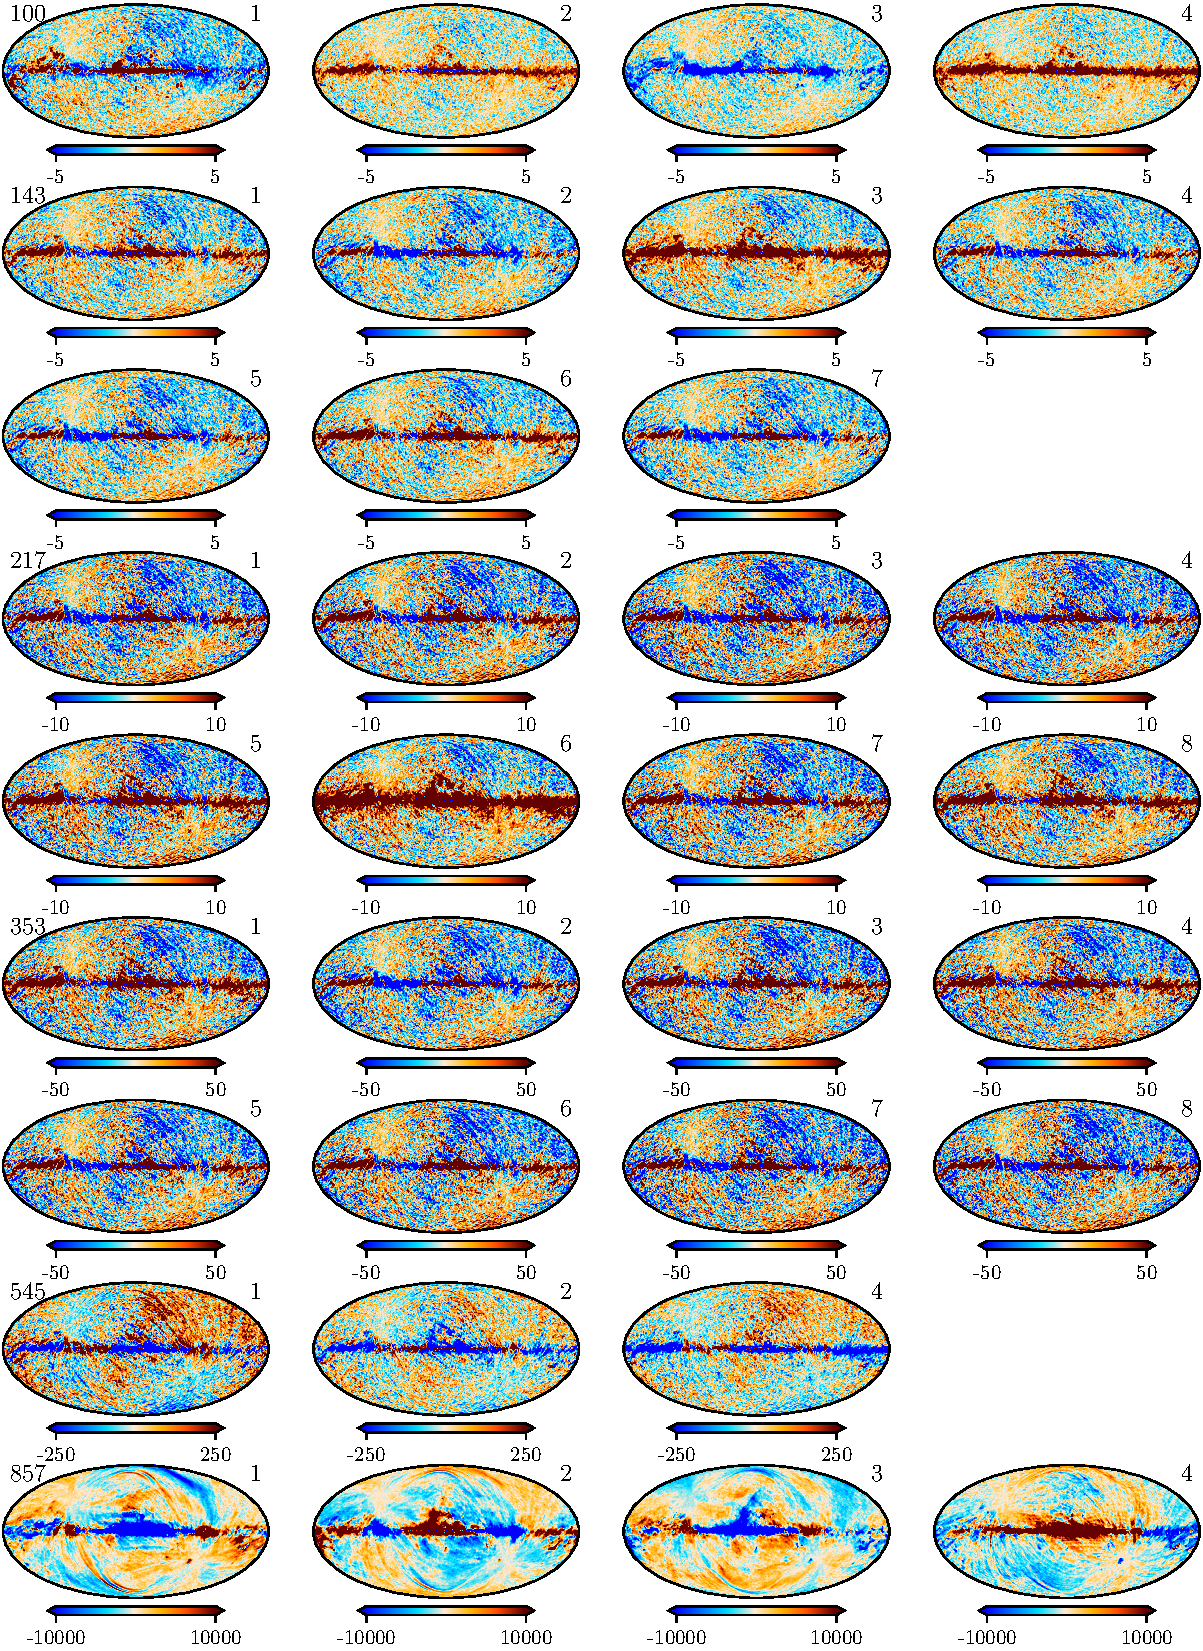
\includegraphics[width=0.85\linewidth]{figures/residuals_plotres.pdf}
    \caption{Residuals (Data minus model) for the \planck\ HFI bands. Units are in $\mu K_\mathrm{CMB}$. The residuals hint at some uncorrected zodiacal light along the ecliptic plane, as well as potentially some offsets to the gain of the 545 channels.}
    \label{fig:residuals}
\end{figure*}


\section{Grid search tests}
\label{app:GridSearchTests}
We plot several of the maps from the grid search in \cref{sec:results}. Since the \Ha\ dust and near dust are templates they do not change by eye (only scaling by a set factor for each frequency given a set of $T,\beta,a$) so they are not plotted here. Thus, we plot the amplitudes of the cold and hot dust for each of the grid points. We show a sample for each of the grids in \cref{fig:SEDGridContours} with the central map the fiducial point and varying the spectral index along the vertical axis and temperature along the y-axis. We do not show values for varying the amplitude scale of the near and \Ha\ dust (\cref{fig:SEDGridAmplitude}) but we found that had negligible effect on the $\chi^2$ and while it does change the correlation with the hot and cold dust we chose to omit them for space considerations. 

\subsection{Cold dust}
As can be seen in \cref{fig:SEDGridContours}, there is an unphysical space mapped by the hottest and highest spectral indices in the cold dust grid. This corresponds to large over-subtraction and negative areas in the hot dust amplitudes as can be seen in \cref{fig:cold_hot_dust_set}.  When shifting the $T_c$ and $\beta_c$ we find the shape of the amplitude maps are visually similar to the fiducial map (see \cref{fig:dust_figures}), so we show the monopole subtracted ratio of the grid position to the fiducial value in \cref{fig:cold_cold_dust_set2}. 
\begin{figure*}[htbp]
    \centering
    \includegraphics[width=\linewidth]{figures/hotDust_cold_Grid.pdf}
    \caption{Hot dust amplitudes for varying $T_\mathrm{c}$ and $\beta_\mathrm{c}$ values with all other grid parameters set to the fiducial values as recorded in \cref{tab:SEDs}. The center panel is the fiducial map. The corresponding cold dust maps ratios can be seen in \cref{fig:cold_cold_dust_set2}. }
    \label{fig:cold_hot_dust_set}
\end{figure*}

% \begin{figure*}
%     \centering
%     \includegraphics[width=\linewidth]{figures/coldDust_cold_Grid.pdf}
%     \caption{Cold dust (\ion{H}{i} correlated dust) amplitudes for varying $T_\mathrm{c}$ and $\beta_\mathrm{c}$ values with all other grid parameters set to the fiducial values as recorded in \cref{tab:SEDs}. The central panel is the fiducial map. The corresponding hot dust maps can be seen in \cref{fig:cold_hot_dust_set}.}
%     \label{fig:cold_cold_dust_set}
% \end{figure*}

\begin{figure*}[htbp]
    \centering
    \includegraphics[width=\linewidth]{figures/coldDust_cold_Grid_ratio.pdf}
    \caption{Monopole subtracted ratio of the cold dust amplitudes compared to the fiducial value (central panel) for varying $T_\mathrm{c}$ and $\beta_\mathrm{c}$. The corresponding hot dust maps can be seen in \cref{fig:cold_hot_dust_set}.}
    \label{fig:cold_cold_dust_set2}
\end{figure*}

\subsection{Hot dust}
Similar to with the cold dust, in \cref{fig:SEDGridContours}, there is an unphysical space mapped by the coldest and lowest spectral index in the hot dust grid. This corresponds to large over-subtraction and negative areas in the cold dust amplitudes as can be seen in \cref{fig:hot_cold_dust_set}. Similar to the cold dust, when shifting the $T_h$ and $\beta_h$ we find the shape of the amplitude maps are visually similar to the fiducial map (see \cref{fig:dust_figures}), so we show the monopole subtracted ratio of the grid position to the fiducial value in \cref{fig:hot_hot_dust_ratio}.
% \begin{figure*}
%     \centering
%     \includegraphics[width=\linewidth]{figures/hotDust_hot_Grid.pdf}
%     \caption{Hot dust (\ion{C}{ii} correlated dust) amplitudes for varying $T_\mathrm{H}$ and $\beta_\mathrm{H}$ values with all other grid parameters set to the fiducial values as recorded in \cref{tab:SEDs}. The center panel is the fiducial map. The corresponding cold dust maps can be seen in \cref{fig:hot_cold_dust_set}. }
%     \label{fig:hot_hot_dust_set}
% \end{figure*}

\begin{figure*}[htbp]
    \centering
    \includegraphics[width=\linewidth]{figures/coldDust_hot_Grid.pdf}
    \caption{Cold dust amplitudes for varying $T_\mathrm{h}$ and $\beta_\mathrm{h}$ values with all other grid parameters set to the fiducial values as recorded in \cref{tab:SEDs}. The central panel is the fiducial map. The corresponding hot dust maps ratios can be seen in \cref{fig:hot_hot_dust_ratio}.}
    \label{fig:hot_cold_dust_set}
\end{figure*}

\begin{figure*}[htbp]
    \centering
    \includegraphics[width=\linewidth]{figures/hotDust_hot_Grid_ratio.pdf}
    \caption{Monopole subtracted ratio of the hot dust amplitudes compared to the fiducial value (central panel) for varying $T_\mathrm{h}$ and $\beta_\mathrm{h}$. The corresponding cold dust maps can be seen in \cref{fig:hot_cold_dust_set}}
    \label{fig:hot_hot_dust_ratio}
\end{figure*}

\subsection{Near Dust}
The nearby dust was found to have unphysical regions banded both by the cold dust amplitudes and the hot dust amplitudes. We additionally aimed to minimized correlations between the cold and near, and hot and near, dust, such that the dust population described by the nearby dust was an independent dust component. For regions with lower $\beta_\mathrm{near}$ and lower $T_\mathrm{near}$ the cold dust starts to behave unphysically and this corresponds also to a higher correlation between the near dust and the hot dust (as can be seen by eye in the lower left panels of \cref{fig:near_hot_dust_set}). 
Conversely, for regions with higher $\beta_\mathrm{near}$ and higher $T_\mathrm{near}$ the hot dust starts to behave unphysically and this corresponds also to a higher correlation between the near dust and the cold dust (as can be seen by eye in the upper right panels of \cref{fig:near_cold_dust_set}). 

% As can be seen in \cref{fig:near_cold_dust_set,fig:near_hot_dust_set} the hottest points in the nearby dust grid lead to high correlations with the hot dust and anti-correlations with the cold dust, and vise versa for the coldest points. 

\begin{figure*}[htbp]
    \centering
    \includegraphics[width=\linewidth]{figures/hotDust_near_Grid.pdf}
    \caption{Hot dust amplitudes for varying $T_\mathrm{near}$ and $\beta_\mathrm{near}$ values with all other grid parameters set to the fiducial values as recorded in \cref{tab:SEDs}. The center panel is the fiducial map. The corresponding cold dust maps can be seen in \cref{fig:near_cold_dust_set}. }
    \label{fig:near_hot_dust_set}
\end{figure*}

\begin{figure*}[htbp]
    \centering
    \includegraphics[width=\linewidth]{figures/coldDust_near_Grid.pdf}
    \caption{Cold dust amplitudes for varying $T_\mathrm{near}$ and $\beta_\mathrm{near}$ values with all other grid parameters set to the fiducial values as recorded in \cref{tab:SEDs}. The central panel is the fiducial map. The corresponding hot dust maps can be seen in \cref{fig:near_hot_dust_set}.}
    \label{fig:near_cold_dust_set}
\end{figure*}


\subsection{\texorpdfstring{H$\alpha$}{Ha} dust}
The parameter space explored for the \Ha\ correlated dust was shown to have a very flat $\chi^2$ profile, and minimal changes to the hot and cold dust amplitudes or correlations. As such we chose to take the DIRBE fit values from \cite{CG02_05} for our fiducial values, as we expect the DIRBE bands to have better control of these SED parameters. 
\begin{figure*}[htbp]
    \centering
    \includegraphics[width=\linewidth]{figures/hotDust_wham_Grid.pdf}
    \caption{Hot dust amplitudes for varying $T_\mathrm{H\alpha}$ and $\beta_\mathrm{H\alpha}$ values with all other grid parameters set to the fiducial values in \cref{tab:SEDs}. The center panel is the fiducial map. The corresponding cold dust maps can be seen in \cref{fig:hot_cold_dust_set}. This explores only $a_\mathrm{H\alpha}=1$.}
    \label{fig:Ha_hot_dust_set}
\end{figure*}

\begin{figure*}[htbp]
    \centering
    \includegraphics[width=\linewidth]{figures/coldDust_wham_Grid.pdf}
    \caption{Cold dust amplitudes for varying $T_\mathrm{H\alpha}$ and $\beta_\mathrm{H\alpha}$ values with all other parameters set to the fiducial values. The central panel is the fiducial map. The corresponding hot dust maps can be seen in \cref{fig:Ha_hot_dust_set}.}
    \label{fig:Ha_cold_dust_set}
\end{figure*}

\begin{figure*}[htbp]
    \centering
    \includegraphics[width=\linewidth]{figures/hotDust_wham_Grid_ratio.pdf}
    \caption{Monopole subtracted hot dust amplitudes ratios compared to the fiducial map (central panel) for varying $T_\mathrm{H\alpha}$ and $\beta_\mathrm{H\alpha}$ values with all other grid parameters set to the fiducial values as recorded in \cref{tab:SEDs}. The corresponding cold dust maps can be seen in \cref{fig:Ha_cold_dust_set_r}.}
    \label{fig:Ha_hot_dust_set_r}
\end{figure*}

\begin{figure*}[htbp]
    \centering
    \includegraphics[width=\linewidth]{figures/coldDust_wham_Grid_ratio.pdf}
    \caption{Monopole subtracted cold dust amplitudes ratios compared to the fiducial map (central panel) for varying $T_\mathrm{H\alpha}$ and $\beta_\mathrm{H\alpha}$ values with all other grid parameters set to the fiducial values as recorded in \cref{tab:SEDs}. The corresponding hot dust maps can be seen in \cref{fig:Ha_hot_dust_set_r}.}
    \label{fig:Ha_cold_dust_set_r}
\end{figure*}

\section{Thermal dust map characterization}
\label{app:dustCharacterization}
We compare the fraction of each dust component contributing to the total in \cref{fig:dustFrac}. As the \Ha\ dust is a dust extinction (with negative amplitude) it contributes a negative fraction to the final, and is the smallest contributor to the total. The near dust dominates outside the plane of the galaxy (which is to be expected, since further dust will be closer to the galactic plane due to geometry). The hot dust is clustered near the galactic center and shows some anti-correlation with the \Ha\ dust. Finally, the cold dust is dominant in the galactic plane further from the galactic center. This further cements the notion that this updated dust model is more physical motivated than previous models, tracing known physical regions within the Milky Way Galaxy. 

\begin{figure*}[htbp]
    \centering
    \includegraphics[width=0.9\linewidth]{figures/dustFrac_plcmap.pdf}
    \caption{Average dust from each component contributing to the total dust signal. }
    \label{fig:dustFrac}
\end{figure*}


\end{document}
%%%% End of aa.dem


% \begin{figure}
%   \centering
%   \includegraphics[width=\columnwidth]{figures/chisq_353_alpha.pdf}
%   \caption{$\chi^2$ distribution for $\alpha$, the conversion factor from GAIA-based extinction to thermal dust emission at 545\,GHz, as evaluated from \Planck\ 353\,GHz data. The dashed vertical line indicates the best-fit value, and the dotted lines indicate the uncertainties. }
%   \label{fig:chisq_353_alpha}
% \end{figure}

% \begin{figure}
%   \centering
%   \includegraphics[width=\columnwidth]{figures/res_353-1_alpha097.pdf}\\
%   \includegraphics[width=\columnwidth]{figures/res_353-1_alpha099.pdf}\\
%   \includegraphics[width=\columnwidth]{figures/res_353-1_alpha101.pdf}
%   \caption{Residual maps at 353\,GHz as a function of $\alpha$. The middle panel corresponds to the best-fit value found in Fig.~\ref{fig:chisq_353_alpha}, while the upper and lower panels correspond to $\pm2\sigma$ deviations.}
%   \label{fig:res_353_alpha}
% \end{figure}


% \begin{figure}
%   \centering
%   \includegraphics[width=\columnwidth]{figures/res_100-1_1deg_v1.pdf}\\
%   \includegraphics[width=\columnwidth]{figures/res_143_1deg_v1.pdf}\\
%   \includegraphics[width=\columnwidth]{figures/res_217-1_1deg_v1.pdf}\\
%   \includegraphics[width=\columnwidth]{figures/res_545_1deg_v1.pdf}
%   \caption{Residual maps for each \Planck\ frequency channel that is included in the fit, evaluated for the best-fit scaling factor of $\alpha=625\,\mu\mathrm{K}_{\mathrm{CMB}}/\mathrm{ext}$. For the 100 and 217\,GHz channels, only the first horn maps are shown for brevity; the others appear visually similar.}
%   \label{fig:res_353_alpha}
% \end{figure}


% \begin{figure*}
%   \centering
%   \includegraphics[width=0.49\textwidth]{figures/dust_353-1_c0001_k000003.png}
%   \includegraphics[width=0.49\textwidth]{figures/ratio_353-1_dust_tot_2deg.png}\\
%   \includegraphics[width=0.49\textwidth]{figures/dust_cii_353-1_c0001_k000003.png}
%   \includegraphics[width=0.49\textwidth]{figures/ratio_353-1_dust_cii_tot_2deg.png}\\
%   \includegraphics[width=0.49\textwidth]{figures/hotPAH_353-1_c0001_k000003.png}
%   \includegraphics[width=0.49\textwidth]{figures/ratio_353-1_hotPAH_tot_2deg.png}
%   \caption{Comparison of the cold (\emph{top}), hot (\emph{middle}), and nearby (\emph{bottom}) thermal dust components as evaluated at 353\,GHz. The left column shows the absolute amplitude on a common linear color scale, while the right column shows the fraction of the given component relative to the sum of the three components. All maps are smoothed to an angular resolution of $2^{\circ}$ FWHM.   }
%   \label{fig:dust_353_ratio}
% \end{figure*}
